\documentclass[12pt,a4paper]{amsart}

\linespread{1.2}
\usepackage{amsmath}
% for bibliography
\usepackage{cite}
\renewcommand{\refname}{\centering References}

%\usepackage{float}
\usepackage{graphicx}

\usepackage{amsmath,amsthm} %for theorems to be with points
\newtheorem{theorem}{Theorem}
\newtheorem{lemma}{Lemma}

\begin{document}

\title{Search for invariant sets of the generalized tent map}

\begin{abstract}
The article uses the predictive control method to search for periodic orbits of the generalized tent map. The main problem is that 
the invariant set containing periodic orbits as a subset is a repeller and set of the Cantor type. Therefore, to find a periodic orbit, 
a simple local stabilization of the orbit may not be enough due to the small measure of the basin of attraction. It is shown that for 
certain values of the control parameter, not only the local behavior of solutions changes in the controlled system, but also the global 
one, namely, an interval or the entire real axis becomes an invariant set. The computational particularities of using the control system 
are considered, the necessary conditions for the found orbit to be periodic are given. The question about local asymptotic stability of 
subcycles of the controlled system's stable cycles is fully investigated. Some statistical properties of the subset of the classical 
Cantor set, which is determined by the periodic points of the generalized tent map, are studied.

\medskip
\noindent \textit{Keywords.} Generalized tent map, predictive control, periodic orbits, local stabilization, invariant sets.  
\end{abstract}


\maketitle

\section*{\centering{Introduction}}

In the seminal paper \cite{Lozi} \textit{R. Lozi} noted that numerical computations using computers play a central role in analyzing 
solutions of nonlinear dynamical systems, that computer-aided proofs are complex and necessarily require additional special 
validation of the results. Nevertheless, numerous researches in the fields related to chaotic dynamical systems are confident 
in the numerical solutions that they found using popular software, with no careful check on the reliability of these results, though 
the researches have to be very cautious to back up theory with numerical computations.

The main computational problem relates to the fact that computers store numbers in registers and memory cells with a limited 
number of digits, which results in the system of real numbers represented in the machine being discrete and finite. To trace what 
consequences can arise because of this, let us consider an example of the computation of an iterated sequence using the standard 
tent function $f(x)=2\cdot\left(\frac12-|x-\frac12|\right)$ in the EXCEL software environment. Choose the initial point $x_0=\frac23.$
Then, theoretically, it must be that $f^{(k)}(x_0)=x_0,$ $k=1,\,2,\,\ldots$ (hereinafter we use the notations $f^{(1)}(x)=f(x),$ 
$f^{(k)}(x)=f\left(f^{(k-1)}(x)\right)$). However, the calculations give different results: $f^{(53)}(x_0)=1,$ $f^{(54)}(x_0)=0.$ 
The first impression is that the problem arose because the number $\frac23$ cannot be represented as a finite decimal fraction. Then 
choose $x_0=0.4.$ Theoretically, there must be $f^{(1)}(x_0)=0.8,$ $f^{(2)}(x_0)=0.4,$ and so on. Yet, as a result of the calculations, 
we again obtain $f^{(53)}(x_0)=1,$ $f^{(54)}(x_0)=0.$ The same results we will also get doing calculations in the MAPLE package, 
if we set $x_0=HFloat(evalf(2/3))$ or $x_0=HFloat(0.4).$ There may be chosen other initial values for $x_0$, and again we will obtain
$f^{(54)}(x_0)=0.$

The reason of such incorrect computations is explained by the fact that a number from the interval $[0,\,1]$ is represented 
in the computer in the binary system by a finite sum of numbers of the form $\frac{\alpha_j}{2^j}$ $\left(\alpha_j\in\{0,1\}\right),$
that is, it is a dyadic rational number equal to $\frac{A}{2^m}$ ($A$ is an integer, and $0\leq A \leq 2^m$). The number $m$ is called 
the exponent. But then $f\left(\frac{A}{2^m}\right)=\frac{A_1}{2^{m-1}}$ ($A_1$ is an integer, and $0\leq A_1 \leq 2^{m-1}$), 
$f^{(2)}\left(\frac{A}{2^m}\right)=\frac{A_2}{2^{m-2}},$ \ldots, $f^{(m+1)}\left(\frac{A}{2^m}\right)=0.$ On the computers 
where computations of iterated sequence were done, the maximum exponent was found to be 53.  

Let us note some properties of dyadic rational numbers \cite{Curtis}. Dyadic rational numbers are closed under addition, subtraction, 
and multiplication, but not division. Dyadic rational numbers form an everywhere dense set on the real line. As a data type used by 
computers, floating-point numbers are often defined as integers multiplied by positive or negative powers of two, and thus all the 
numbers, that can be represented, for example, in the IEEE floating-point format, are dyadic rationals. The same is true for most data 
types with a fixed point.

The majority of computer applications provide the representation of numbers in a convenient readable form, i.e. in decimal notation. 
However, the problem of incorrect computations does not disappear. So in the MAPLE package, at $x_0=evalf(\frac23)$ the calculated 
iterated sequence will differ considerably from the theoretical one, in which $f^{(k)}(x_0)=x_0,$ $k=1,\,2,\,\ldots$. Although when 
$x=0.4,$ we will actually obtain a sequence of alternating numbers 0.4 and 0.8. 

To show that the problem lies not in the numeral system used by the program for calculations, consider the function
$$f_h(x)=
\left\{\begin{array}{ll}
hx-2j,\,x\in\left[\frac{2j}{h},\frac{2j+1}{h}\right],\;j=0,\ldots,\left[\frac{h}{2}\right]-1, \\
-hx+2j+2,\,x\in\left[\frac{2j+1}{h},\frac{2j+2}{h}\right],\;j=0,\ldots,
\lfloor{\frac{h}{2}}\rfloor-1,
\end{array}\right.$$
where $h$ is a natural number (the graph of the function $f_{10}(x)$ is shown in Fig. 1). Suppose that a computer program uses 
the numeral system with the base $h$ to represent numbers. Then for any $x_0\in[0,\,1],$ there will exist a number $m$ (the 
maximum exponent) such that $f_h^{(m+1)}(x_0)=0.$ That is, the computations will be performed, generally speaking, not correctly.
So, setting $x_0$ with a decimal fraction in the MAPLE package, and assigning the value $\mu$ to the Digits variable (the number of 
decimal places used), would give us $f_{10}^{(\mu+1)}(x_0)=0.$

% Figure 1
\begin{figure}[h!]
\centering
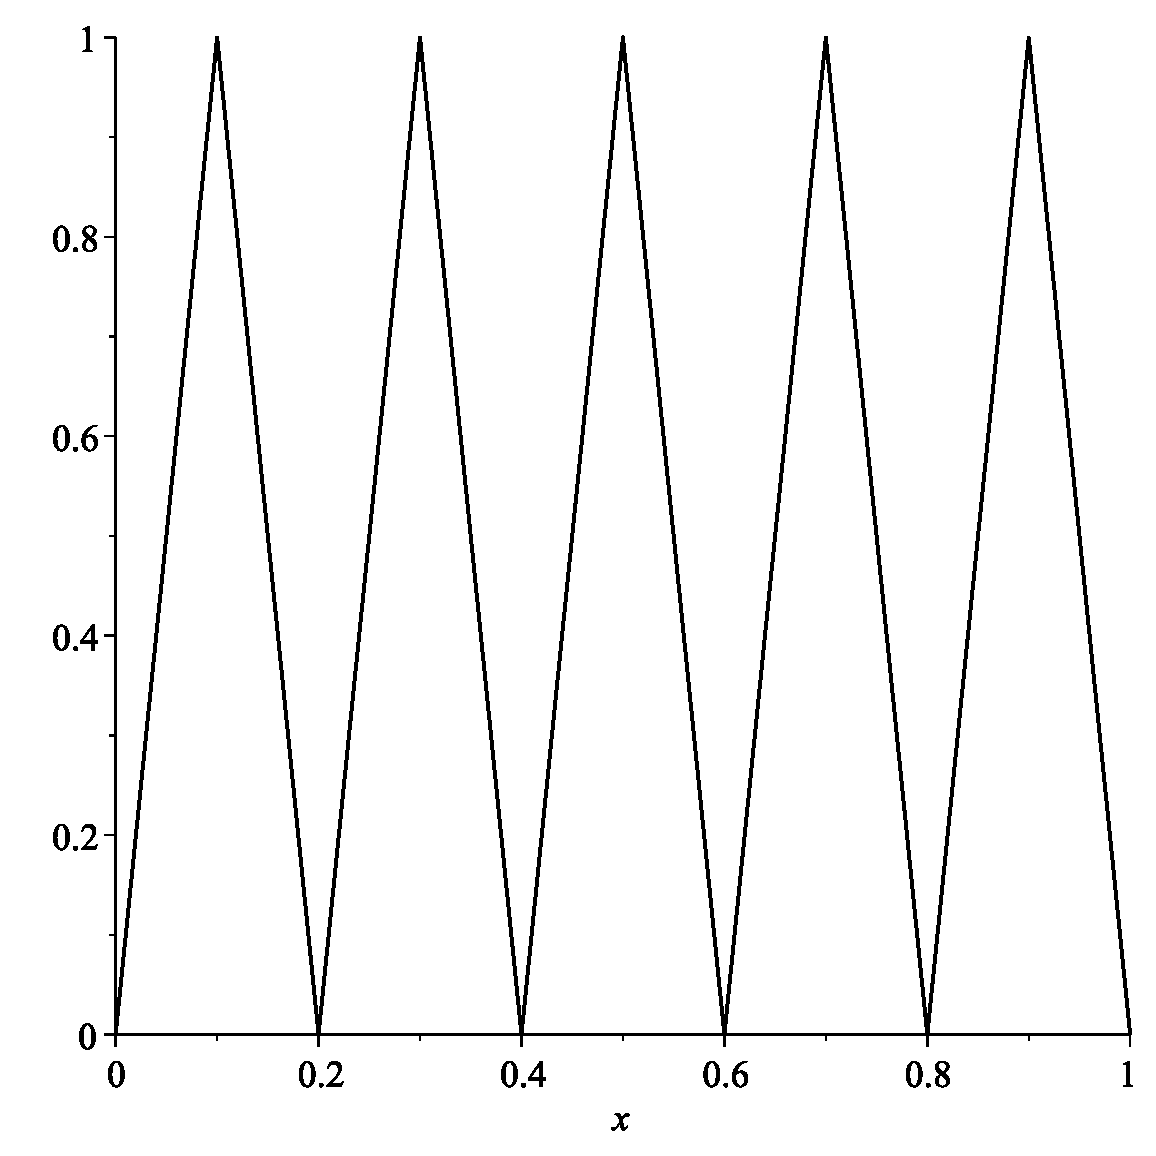
\includegraphics[scale=0.28]{Fig1}
\caption{Graph of the function $f_{10}(x)$.} \label{f1}
\end{figure}

Moreover, it is easy to show that any rational fraction from the interval $[0,\,1]$ is a periodic or preperiodic point of the map $f_h(x).$
Indeed, under this mapping, a rational fraction goes into a rational fraction with the same denominator, and there are a finite number 
of proper fractions with the same denominator. That is, if the calculations are performed correctly, then the sequence iterated using 
the mapping $f_h(x)$ must be periodic (at least starting from some number). 

Let $\nu$ be an integer and the base of the numeral system in which the computer program performs calculations. The sequence 
iterated with the help of the map $f_h(x)$ will be computed correctly if and only if $\nu\neq h,$ and the initial point $x_0$ is representable 
in the form of $\frac{A}{\nu^m}$ ($A$ is an integer, and $0\leq A\leq \nu^m$). 

Let us consider one more example. Take the shifted tent function  
$$f(x)=
\left\{\begin{array}{ll}
3x,\,x\leq\frac13, \\
\frac32(1-x),\,x>\frac13.
\end{array}\right.$$
For the initial value $x_0=0.4,$ compute the iterated sequence using the EXCEL environment and the MAPLE package. If setting 
$x_0=HFloat(0.4)$ in MAPLE, we will get a sequence that coincides with the sequence in EXCEL. If in the MAPLE package we set $x_0$ 
by a decimal fraction and assign to the Digits variable the value 50, for instance, then we will obtain a completely different sequence. 
So in EXCEL and MAPLE with binary representation of numbers $x_{49}=0.1490...,$ but in MAPLE with decimal representation
$x_{49}=0.1488...$ . Upon further calculation, we can observe a significant divergence between the elements of these sequences 
(for example, the corresponding values at the step 70 are 0.661... and 0.989...). Moreover, let us calculate this sequence in the MAPLE 
package with decimal representation when the Digits variable value is 50 and 100. At the three hundredth step, we will get, correspondingly: 
$x_{300}=0.395...$ and $x_{300}=0.930...$ . Such divergences are due to the fact that with an increase in the number of iterations, 
the number of significant decimal digits after the decimal point in the sequence elements increases, and once their number exceeds the 
calculation accuracy declared by the Digits variable, further iterations will be performed incorrectly.

Finally, consider the logistic map $f(x)=4x(1-x).$ We will carry out the computations in the MAPLE package with decimal representation 
at the value of the Digits variable equal to 50 and 100. In the first case, the sequence $\left\{x_k=f^{(k)}(x_0)\right\}$ will be generated, 
in the second one -- the sequence $\left\{y_k=f^{(k)}(y_0)\right\},$ $k=1,\,2,\ldots.$ Set $x_0=y_0=0.4$ and construct the sequence 
$\{x_k-y_k\}.$ Let us picture it on the graph (Fig. 2). It can be seen that, starting from the step 170, the behavior of this sequence is 
quasi-stochastic. 

% Figure 2
\begin{figure}[h!]
\centering
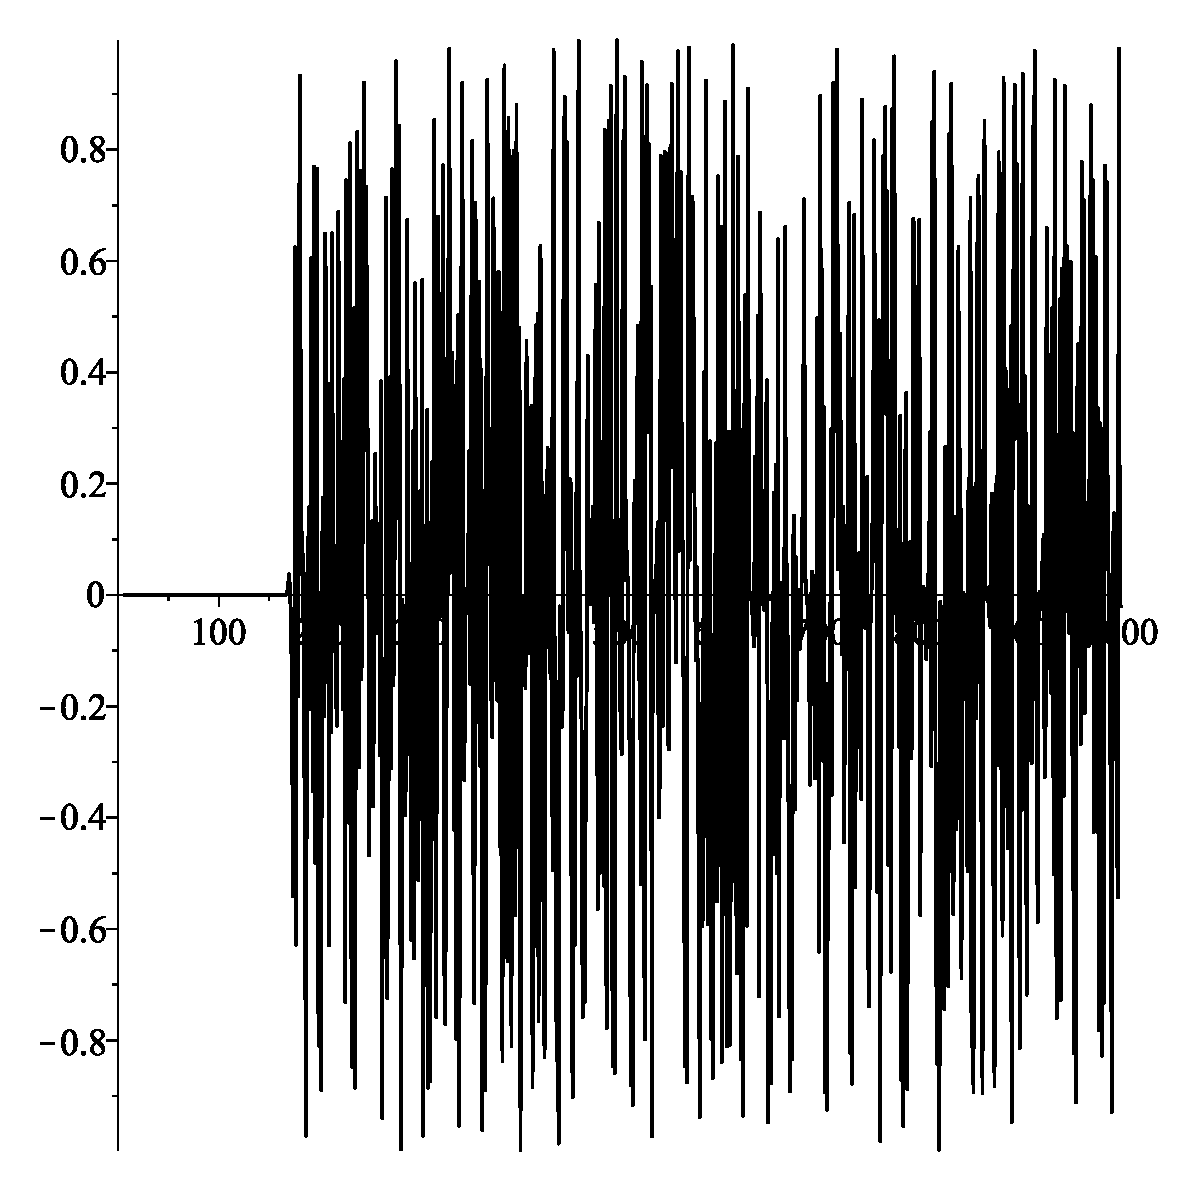
\includegraphics[scale=0.28]{Fig2a}
\hspace{1cm}
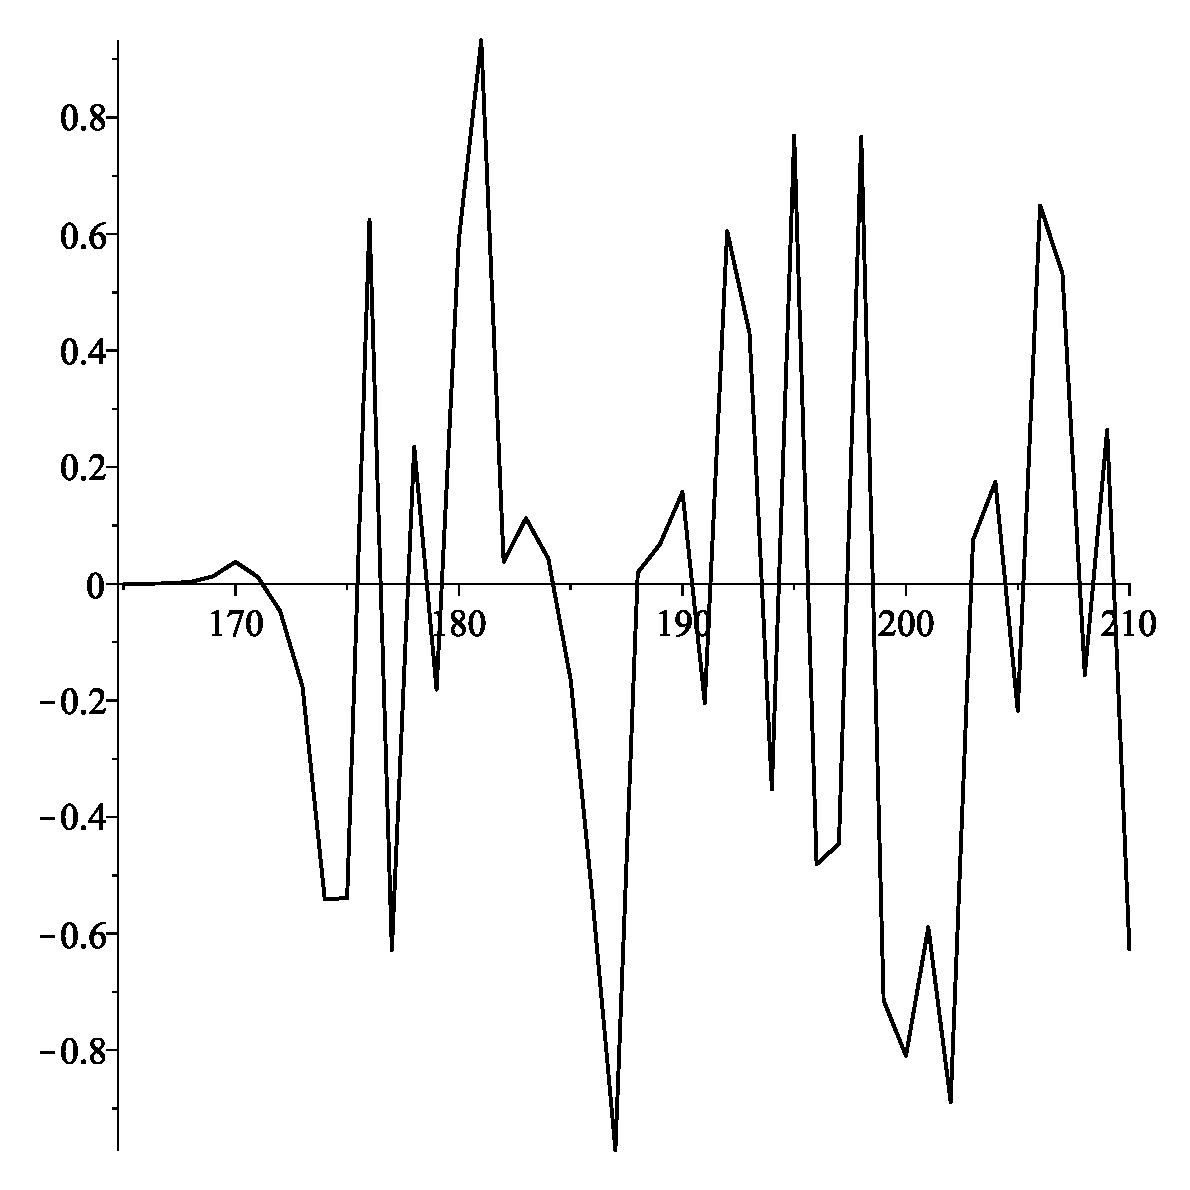
\includegraphics[scale=0.28]{Fig2b}
\caption{Graphical representation of the sequence $\{x_k-y_k\}$ \\\centering 
a) at $k=1,\,\ldots,\,1000$ \hspace{1cm}
b) at $k=165,\,\ldots,\,210$} \label{f2}
\end{figure}

We can continue giving similar examples. However, the above examples already clearly show that a researcher can never be sure 
of the correctness of calculations made on a computer. That is, the answer to \textit{R.~Lozi}'s question about trust in the numerical 
results is, unfortunately, negative. This once again proves the need to develop mathematical methods enabling us to correct computer 
calculations. Naturally, each such method will depend on the specifics of the problem that is being solved.  

In the present article, it will be shown how we can correct the computational procedure in the problem of finding periodic orbits 
of a nonlinear discrete system on the example of the tent map. 

The dynamics of even the simplest nonlinear discrete systems can be quite complex \cite{Devaney, Chen, Andr}. Such systems are often characterized 
by extremely unstable motions in phase space, which are defined as chaotic \cite{Devaney}. In dissipative systems, these motions define invariant sets, 
which can be strange attractors or repellers. Trajectories on such invariant sets have positive Lyapunov exponents; therefore, these 
trajectories are exponentially sensitive to the initial conditions. Invariant sets can be studied by considering unstable periodic orbits, 
which constitute the framework of these invariant sets. Periodic orbits have a hierarchical structure determined by their length, which 
makes it possible to calculate various characteristics of invariant sets and their subsets, for example, topological dimension and entropy \cite{Biham}. 
However, applying numerical methods of searching for periodic orbits (periodic points that determine the orbit) encounters a number 
of fundamental problems. Due to the sensitivity to initial conditions and rounding errors, after several calculation steps, the results can 
vary greatly depending on the chosen calculation accuracy, the so-called ``butterfly effect'' occurs. Even with a real possibility to choose 
a very high accuracy of calculations, we will never be able to say with certainty what we actually found: a long cycle, a pseudo-cycle or 
a strange attractor \cite{Lozi}.

There exist various methods of searching for periodic orbits of a nonlinear discrete system, which can be divided into two groups: methods 
that do not use the correction of the original discrete dynamical system, for example, the method of interval arithmetic analysis \cite{Zyg, Gal2002, Gal2001}, 
the method connected with the construction of special Hamiltonian systems \cite{Biham}; and methods based on local stabilization of 
an unknown periodic orbit of a given length \cite{Ott, Qian, Aleks, Yang, Miller, DSLS}. The second group of methods is more preferable in the sense that with the growth 
of calculations, their accuracy increases due to the correction of the original dynamical system. If with the help of the control action we 
can locally stabilize the orbit, then the trajectories of the system will remain in the neighborhood of the orbit and will be attracted to it, 
i.e. the periodic orbit will be found. By choosing different initial points, different periodic orbits can be found. To solve the problems of 
stabilization and search of periodic orbits, there were proposed various control schemes that use information about the states of the controlled 
system at previous points in time \cite{Pyr, Vie, DK, Mor} (delayed control) or about the states of the initial system at future points in time \cite{Polyak, Ushio, Shal, DSI} 
(predictive control). 

The purpose of this article is to illustrate the effectiveness of the predictive control method using the example of the generalized tent map. 
The invariant sets of the generalized tent map are repellers that have the structure of the Cantor set. It is shown that in a controlled system, 
along with a change in the local behavior of solutions, the global behavior also changes. The invariant sets of the controlled system have been found, 
this is either an interval or the union of intervals. Locally asymptotically stable periodic orbits are subsets of the invariant set. The basins of 
attraction of these orbits are estimated. 

The paper is organized as follows. In Section~1, we present the main Theorem of the work \cite{DSI}, which substantiates the generalized 
predictive control scheme. Section~2 poses the problem of finding a cycle of length $T$, and Section~3 provides necessary and sufficient conditions 
for the local asymptotic stability of this cycle. Section~4 is the main one in the present work, it provides conditions under which all solutions 
of the controlled system are bounded (Theorem~2), or solutions with initial values from a given interval are bounded (Theorem~3). It was also 
noted that the cycles do not lose the property of local asymptotic stability. In the fifth section, some computational particularities of using 
the control system for finding cycles are considered, the necessary conditions for the found periodic sequence to be a cycle are given. 
In the sixth section, using the example of stabilization of cycles of small lengths, we consider the relationship between the geometry of the original 
map and the map determined by the controlled system. In Section~7, the question about local asymptotic stability of subcycles of the controlled 
system's stable cycles is fully investigated (Theorem~4). Section 8 studies subsets of the classical Cantor set. The Cantor set is characterized by 
points of the first and second type. The points that are end-points of the adjacent to the Cantor set intervals are called points of the first type. 
All the other points of the set are called points of the second type. Among the points of the second type, we can select a subset consisting 
of all cyclic points of the generalized tent map. For specific values of the period, a set of periodic points and a graph of the corresponding 
distribution density function are constructed. The graph is compared with the graph of the density function for the distribution of the Cantor 
set's points of the first type.


%_________________________________________________________________________________
\section{\centering{Preliminary results}}

We consider the nonlinear discrete system 

\begin{equation}\label{sys}
x_{n+1}=f(x_n),\;x_n\in R^m,\;n=1,\,2,\ldots,
\end{equation}
where $f(x)$ is a differentiable vector function of the corresponding dimension. It is assumed that this system has one or several unstable 
$T$-cycles $\left(\eta_1,\ldots,\,\eta_T\right),$ where all the vectors $\eta_1,\ldots,\,\eta_T$ are different, i.e. $\eta_{j+1}=f(\eta_j),$ 
$j=1,\ldots,\,T-1,$ $\eta_1=f(\eta_T).$ Cycle vectors are called cyclic points and constitute a periodic orbit. The multipliers of the considered
unstable cycles are defined as the eigenvalues of the products of Jacobi matrices $\prod\limits_{j=1}^T{f'(\eta_{T-j+1})}$ of dimension 
$m\times m$ at the points of the cycle. The matrix $\prod\limits_{j=1}^T{f'(\eta_{T-j+1})}$ is called the Jacobi matrix of the cycle 
$\left(\eta_1,\ldots,\,\eta_T\right).$ The collection of all multipliers $\left\{\mu_1,\ldots,\,\mu_m\right\}$ is called the spectrum of 
the Jacobi matrix. As a rule, the cycles $\left(\eta_1,\ldots,\,\eta_T\right)$ of system~(\ref{sys}) are not known a priori. Consequently, 
the spectrum is not known either.

Consider the control system	
\begin{equation}\label{csys}
x_{n+1}=f\left(\vartheta_1 x_n + \sum\limits_{j=2}^N{\vartheta_j f^{\left((j-1)T\right)}}(x_n)\right).
\end{equation}
The numbers $\vartheta_1,\ldots,\,\vartheta_N$ are real. It is easy to verify that when $\sum\limits_{j=1}^N{\vartheta_j}=1,$ 
system~(\ref{csys}) also has a cycle $\left\{\eta_1,\ldots,\,\eta_T\right\}.$ The problem is to choose a parameter $N$ 
and coefficients $\vartheta_1,\ldots,\,\vartheta_N$ so that the cycle $\left\{\eta_1,\ldots,\,\eta_T\right\}$ of system~(\ref{csys}) 
is locally asymptotically stable.

\begin{theorem}[\cite{DSI} ]\label{th1}
Suppose $f\in C^1$ and that system~(\ref{sys}) has an unstable $T$-cycle with multipliers $\left\{\mu_1,\ldots,\,\mu_m\right\}.$
Then this cycle will be a locally asymptotically stable cycle of system~(\ref{csys}) if 
$$
\mu_j \left[r(\mu_j)\right]^T \in D,\;j=1,\ldots,\,m,
$$
where $D=\left\{z\in C:\;|z|<1\right\}$ is an open central unit disc on the complex plane, $r(\mu)=\sum\limits_{j=1}^N{\vartheta_j \mu^{j-1}}.$
\end{theorem}



%_________________________________________________________________________________
\section{\centering{Problem statement}}

Consider the nonlinear discrete-time equation
\begin{equation}\label{eq}
x_{n+1}=f(x_n),\;n=1,\,2,\ldots,
\end{equation}
where 
\begin{equation}\label{tent}
f(x)=H\left(\frac12-\left|x-\frac12\right|\right)=
\left\{\begin{array}{ll}
Hx,\,x\leq\frac12, \\
H(1-x),\,x>\frac12,
\end{array}\right.
\end{equation}
$x\in(-\infty;+\infty),$ $H>2.$ The map~(\ref{tent}) is called the tent map. Note that, despite the relative simplicity of function~(\ref{tent}), 
equation~(\ref{eq}) is of great theoretical importance and can also be used to solve some applied problems \cite{Derr, Goh}.

A set $U$ is called invariant for equation~(\ref{eq}) if for any $x_0\in U$ it follows that $f^{(k)}(x_0)\in U,$ $k=1,\,2,\ldots\,.$ It is shown in \cite{Leonov}
that at $H=3$ the invariant set of equation~(\ref{eq}) is the classical Cantor set. Analogously, it can be shown that when $H>2,$ the equation~(\ref{eq}) 
invariant set is a set of the Cantor type, that is: closed, with cardinality of the continuum, with zero Lebesgue measure. Note that each point of the invariant 
set can be represented in the form $\sum\limits_{j=1}^{\infty}{\frac{\alpha_j}{H^j}},$ where $\alpha_j\in\{0,\,H-1\}.$ This set includes a countable subset 
of all periodic points of map~(\ref{tent}). If $x_0$ does not belong to the invariant set, then the corresponding sequence 
$\left\{f^{(k)}(x_0)\right\}_{k=1}^{\infty}$ tends to $-\infty.$ Such invariant sets are called repellers of map~(\ref{tent}). The set 
$\left\{\eta_1,\ldots,\,\eta_T\right\}$ is called a $T$-cycle of map~(\ref{tent}), if the numbers $\eta_1,\ldots,\,\eta_T$ are different, and 
$\eta_{j+1}=f(\eta_j),$ $j=1,\ldots,\,T-1,$ $\eta_1=f(\eta_T),$ and in this case, each point of the $T$-cycle is called a $T$-periodic point. The problem is: 
for given $T$, to find $T$-periodic points of map~(\ref{tent}).



%_________________________________________________________________________________
\section{\centering{Control system and local behavior of the control system trajectories}}

To solve the stated problem, we will use the predictive control method. Along with equation~(\ref{eq}), consider the equation
\begin{equation}\label{ceq}
x_{n+1}=F(x_n),\;n=1,\,2,\ldots,
\end{equation}
where $F(x)=f\left(\vartheta x + (1-\vartheta)f^{(T)}(x)\right),$ $\vartheta$ is some real number, called the control parameter and to be determined later.
Equation~(\ref{ceq}) we will call the control system for equation~(\ref{eq}). 

Let $\left\{\eta_1,\ldots,\,\eta_T\right\}$ be the equation~(\ref{eq}) cycle. Since $\vartheta \eta_k + (1-\vartheta)f^{(T)}(\eta_k)=\eta_k,$ then 
$F(\eta_k)=f(\eta_k),$ which means that the cycle of the equation~(\ref{eq}) will also be the cycle of equation~(\ref{ceq}). Note that the converse statement 
is generally not true. 

The multiplier of the equation~(\ref{eq}) cycle is defined by the formula
$$
\mu = f'(\eta_T)\cdot\ldots\cdot f'(\eta_1). 
$$
Since $\left|f'(\eta_j)\right|=H,$ then $|\mu|=H^T>1,$ that is, any cycle of equation~(\ref{eq}) is unstable. Let us find the value of the multiplier 
$\lambda$ of the same cycle $\left\{\eta_1,\ldots,\,\eta_T\right\},$ but for equation~(\ref{ceq}). From \textit{Theorem~\ref{th1}} we get that 
$$
\lambda=\mu \left(\vartheta+(1-\vartheta)\mu\right)^T. 
$$

In what follows, we will separate two cases: $\mu>0$ and $\mu<0.$ Let $\mu=H^T.$ Then the condition for local asymptotic stability 
of the $T$-cycle of equation~(\ref{ceq}) is: $|\lambda|=\left|H^T \left(\vartheta + (1-\vartheta)H^T\right)^T\right|<1,$ 
from which it follows that 
\begin{equation}\label{inp}
1<
\frac{H^T-\frac{1}{H}}{H^T-1}<
\vartheta<
\frac{H^T+\frac{1}{H}}{H^T-1}<
\frac52.
\end{equation}

If $\mu=-H^T,$ then the condition for local asymptotic stability of the equation~(\ref{ceq}) cycle is: 
$|\lambda|=\left|H^T \left(\vartheta - (1-\vartheta)H^T\right)^T\right|<1,$
from which 
\begin{equation}\label{inn}
\frac12<
\frac{H^T-\frac{1}{H}}{H^T+1}<
\vartheta<
\frac{H^T+\frac{1}{H}}{H^T+1}<
1.
\end{equation}

\begin{lemma}\label{l1}
Given a $T$-cycle of equation~(\ref{eq}) with the multiplier $\mu.$ This cycle will be a locally asymptotically stable cycle of 
equation~(\ref{ceq}) if inequalities~(\ref{inp}), in the case $\mu>0,$ or inequalities~(\ref{inn}), when $\mu<0,$ are satisfied.
\end{lemma}



%_________________________________________________________________________________
\section{\centering{Global behavior of the control system trajectories}}

If there are locally asymptotically stable cycles in equation~(\ref{ceq}), then the invariant set of this equation also includes the basins of 
attraction of these cycles. Since the basin of attraction of a cycle is an open set, its measure is positive. However, there remains the question 
about how large this measure is. This question is important for choosing the initial point for which the corresponding orbit should eventually 
get into the basin of attraction the desired cycle. Thus, as we passing from equation~(\ref{eq}) to equation~(\ref{ceq}), there is ensured a change 
in the nature of the periodic orbit (the set of points of the cycle) which turns from a repeller into an attractor, but it is also important 
to additionally provide a sufficiently large measure of the basin of attraction. 

Below we will establish the properties of invariant sets of equation~(\ref{ceq}) and the global behavior of its solutions. 
The properties are formulated as lemmas. From these properties, two main theorems, allowing us to find all cycles of arbitrary 
lengths with any given accuracy, will follow. 

\begin{theorem}\label{t2}
If inequalities $\frac{H^T-\frac{1}{H}}{H^T-1}<\vartheta\leq\frac{H^T+\frac1H}{H^T-1}$ are satisfied, then any solution of equation~(\ref{ceq}) is bounded. Moreover, any $T$-cycle $\left\{\eta_1,\ldots,\,\eta_T\right\}$ 
of this equation, for which the quantity $\mu = f'(\eta_T)\cdot\ldots\cdot f'(\eta_1)$ is positive, is locally asymptotically stable.
\end{theorem}

\begin{theorem}\label{t3}
If the inequalities $\frac{H^T-\frac{1}{H}}{H^T+1}<\vartheta\leq\frac{H^T}{H^T+1}$ are satisfied, the set $\left[0,\,\frac{H}{2}\right]$ is an invariant set
of equation~(\ref{ceq}). Moreover, any $T$-cycle $\left\{\eta_1,\ldots,\,\eta_T\right\}$ of this equation, for which the quantity 
$\mu = f'(\eta_T)\cdot\ldots\cdot f'(\eta_1)$ is negative, is locally asymptotically stable.
\end{theorem}

We proceed to formulate and prove the main lemmas.

Let inequalities~(\ref{inp}) be satisfied. Divide conditions~(\ref{inp}) into three cases: $\vartheta=\frac{H^T}{H^T-1},$
$\frac{H^T-\frac{1}{H}}{H^T-1}<\vartheta<\frac{H^T}{H^T-1},$ $1<\frac{H^T}{H^T-1}<\vartheta<\frac{H^T+\frac{1}{H}}{H^T-1}.$

\begin{lemma}\label{l2}
Let $\vartheta=\frac{H^T}{H^T-1}.$ Then, if $x_0\leq 0,$ it follows that $F(x_0)=0,$ hence, $F^{(k)}(x_0)=0$ when $k=1,\,2,\ldots;$
if $x_0\geq 1,$ then $F(x_0)<0,$ hence, $F^{(k)}(x_0)=0$ when $k=2,\,3,\ldots;$ if $x_0\in(0,\,1),$ then 
$\left\{F^{(k)}(x_0)\right\}_{k=2}^{\infty}\in[0,\,1].$  
\end{lemma}

\begin{proof}
Let $x_0\leq 0,$ then $f(x_0)=Hx_0\leq 0,$ $f^{(2)}(x_0)=H^2 x_0\leq 0,$ \ldots, $f^{(T)}(x_0)=H^T x_0.$  Find 
$$
\zeta=\vartheta x_0 + (1-\vartheta)f^{(T)}(x_0)=\frac{1}{H^T-1}\left(H^T x_0 - H^T x_0\right)=0.
$$ 
Hence, $F(x_0)=f(\zeta)=0.$

Let $x_0\geq 1,$ then $f(x_0)=H (1-x_0)\leq 0,$ $f^{(2)}(x_0)=H^2 (1-x_0)\leq 0,$ \ldots, $f^{(T)}(x_0)=H^T (1-x_0),$
$\zeta=\vartheta x_0 + (1-\vartheta)f^{(T)}(x_0)=\frac{1}{H^T-1}\left(H^T x_0 - H^T (1-x_0)\right)=\frac{H^T}{H^T-1}(2x_0-1)>1,$
$F(x_0)=f(\zeta)=H(1-\zeta)<0.$ Hence, $F^{(2)}(x_0)=0.$ 

The last case remains: at $x_0\in(0,\,1),$ either starting from some number $k>k_0,$  $F^{(k)}(x_0)=0,$ or 
$\left\{F^{(k)}(x_0)\right\}_{k=2}^{\infty}\in(0,\,1).$ The lemma is proved.
\end{proof}

The case $\frac{H^T-\frac{1}{H}}{H^T-1}<\vartheta<\frac{H^T}{H^T-1}$ is considered in a similar way.

\begin{lemma}\label{l3}
Let $\frac{H^T-\frac{1}{H}}{H^T-1}<\vartheta<\frac{H^T}{H^T-1}.$ Then, if $x_0\leq 0$ or $x_0\geq 1,$ 
${F^{(k)}(x_0)\xrightarrow[k\rightarrow\infty]{}0;}$ when $x_0\in(0,\,1),$ either $F^{(k)}(x_0)\xrightarrow[k\rightarrow\infty]{}0$
or $\left\{F^{(k)}(x_0)\right\}_{k=1}^{\infty}\in(0,\,1).$
\end{lemma}

\begin{proof}
Let $x_0\leq 0,$ then $f(x_0)=Hx_0\leq 0,$ \ldots, $f^{(T)}(x_0)=H^T x_0.$ Find 
$$
\zeta=\vartheta x_0 + (1-\vartheta)f^{(T)}(x_0)=\left(H^T - \vartheta (H^T - 1)\right)x_0.
$$
It follows from the inequality $\frac{H^T-\frac{1}{H}}{H^T-1}<\vartheta<\frac{H^T}{H^T-1}$ that, first, $\zeta\leq 0,$ 
and $F(x_0)=f(\zeta)=H\zeta=H\left(H^T - \vartheta (H^T - 1)\right)x_0\leq 0,$ and second, 
$0<\alpha = H\left(H^T - \vartheta (H^T - 1)\right)<1,$ from which $F(x_0)=-\alpha|x_0|>-|x_0|.$ Then 
$\left|F^{(k)}(x_0)\right|=\alpha^k |x_0|\xrightarrow[k\rightarrow\infty]{}0.$

Let $x_0\geq 1,$ then $f(x_0)=H(1-x_0)\leq 0,$ \ldots, $f^{(T)}(x_0)=H^T (1-x_0),$
$$
\zeta=\vartheta x_0 + (1-\vartheta)f^{(T)}(x_0)=x_0+(\vartheta-1)\left(x_0 + H^T (x_0-1)\right)>x_0>1.
$$
Then $F(x_0)=f(\zeta)=H(1-\zeta) < 0.$ Hence, $F^{(2)}(x_0)=-\alpha\left|F(x_0)\right|>-\left|F(x_0)\right|,$
$\left|F^{(k)}(x_0)\right|=\alpha^{k-1} \left|F(x_0)\right| \xrightarrow[k\rightarrow\infty]{}0.$

Let $x_0\in(0,\,1).$ If for some $k_0$ $F^{(k_0)}(x_0)\leq 0$ or $F^{(k_0)}(x_0)\geq 1,$ then 
$F^{(k)}(x_0)\xrightarrow[k\rightarrow\infty]{}0.$ Otherwise, $\left\{F^{(k)}(x_0)\right\}_{k=1}^{\infty}\in(0,\,1).$
The lemma is proved. 
\end{proof}

The case $\frac{H^T}{H^T-1}<\vartheta<\frac{H^T+\frac{1}{H}}{H^T-1}$ remains.

\begin{lemma}\label{l4}
Let $\frac{H^T}{H^T-1}<\vartheta<\frac{H^T+\frac{1}{H}}{H^T-1}.$ In this case, if $-H^2+\frac{H}{2}\leq x_0 \leq \frac{H}{2},$ 
then
\begin{equation}\label{inl4}
-H^2+\frac{H}{2}\leq F^{(k)}(x_0) \leq \frac{H}{2},\;k=1,\,2,\ldots\,.
\end{equation}
If $x_0>\frac{H}{2}$ or $x_0<-H^2+\frac{H}{2},$ there exists a number $k_0\leq 0$ such that inequalities~(\ref{inl4}) are satisfied 
for all $k$ greater than $k_0.$ 
\end{lemma}

\begin{proof}
Let $x_0\leq 0,$ then $f(x_0)=Hx_0\leq 0,$ \ldots, $f^{(T)}(x_0)=H^T x_0,$
$$
\zeta=\left(H^T - \vartheta (H^T - 1)\right)x_0.
$$
The inequality $\frac{H^T}{H^T-1}<\vartheta<\frac{H^T+\frac{1}{H}}{H^T-1}$ is equivalent to 
$-\frac{1}{H}<H^T-\vartheta(H^T-1)<0,$ from which it follows that $0\leq\zeta\leq\frac{|x_0|}{H}.$ If $-H\leq x_0\leq 0,$ then 
$0\leq\zeta\leq 1$ and $0\leq F(x_0)\leq \frac{H}{2}.$

If $x_0<-H$ and $\zeta\geq 1,$ then $0\geq F(x_0)=H(1-\zeta)>H-|x_0|.$ Moreover, if $F^{(k)}(x_0)<-H$ and 
$\left(H^T - \vartheta (H^T - 1)\right)F^{(k)}(x_0)\geq 1,$ then $0\geq F^{(k+1)}(x_0)>H-\left|F^{(k)}(x_0)\right|>(k+1)H-|x_0|.$
It means that there exists such $k_0$ that $-H\leq F^{(k_0)}(x_0)\leq 0.$ And hence, $0\leq F^{(k_0+1)}(x_0)\leq\frac{H}{2}.$

Let $0\leq x_0\leq \frac{H}{2},$ then $H^T \left(1-\frac{H}{2}\right)\leq f^{(T)}(x_0)\leq\frac{H}{2}.$ Since $\vartheta>1,$ then
\begin{gather*}
-\frac34 H < \vartheta x_0 - (\vartheta-1)\frac{H}{2} \leq \zeta \leq \vartheta x_0 + (\vartheta-1)H^T\left(\frac{H}{2}-1\right) < \\
< \vartheta\frac{H}{2} + (\vartheta-1)H^T\left(\frac{H}{2}-1\right) <\\
<\frac{1}{H^T-1}\left( \left( H^T+\frac{1}{H} \right)\frac{H}{2} + \left( 1+\frac{1}{H} \right) H^T \left( \frac{H}{2}-1 \right) \right) = \\
=\frac{1}{H^T-1} \left( H^{T+1} - \frac{H^T}{2} - H^{T-1} + \frac12\right).
\end{gather*}
Note that $1<H-1<\frac{1}{H^T-1} \left( H^{T+1} - \frac{H^T}{2} - H^{T-1} + \frac12\right)<H+\frac12.$ Then 
$$
F(x_0) > H\left(1 - \frac{1}{H^T-1} \left( H^{T+1} - \frac{H^T}{2} - H^{T-1} + \frac12\right) \right) > -H\left(H - \frac12\right).
$$
Therefore, if $0\leq x_0\leq \frac{H}{2},$ then $-H^2+\frac{H}{2}\leq F(x_0) \leq \frac{H}{2}.$

Let $x_0 > \frac{H}{2},$ then $f^{(T)}(x_0)=H^T (1-x_0),$  $\zeta=\vartheta x_0 + (\vartheta - 1) H^T (x_0 - 1) > 1,$ and $F(x_0)<0.$
It means that for some $k_0$ the inequality $0 \leq F^{(k_0)}(x_0) \leq \frac{H}{2}$ is satisfied.  

Summing up the above four cases, we get that when $-H^2+\frac{H}{2}\leq x_0 \leq \frac{H}{2},$ inequalities~(\ref{inl4}) hold. 
If $x_0>\frac{H}{2}$ or $x_0<-H^2+\frac{H}{2},$ then inequalities~(\ref{inl4}) will be satisfied starting from some number. 
The lemma is proved. 
\end{proof}

From Lemmas~\ref{l1}, \ref{l2}, \ref{l3}, \ref{l4}, the assertion of Theorem~\ref{t2} follows.

Let us now pass to the study of the global behavior of the $T$-cycles $\left\{\eta_1,\ldots,\,\eta_T\right\}$ of equation~(\ref{ceq}) 
for which the quantity $\mu = f'(\eta_T)\cdot\ldots\cdot f'(\eta_1)$ is negative, assuming that conditions~(\ref{inn}) are satisfied.

\begin{lemma}\label{l5}
Let conditions~(\ref{inn}) be satisfied and $x_0<0.$ Then $F^{(k)}(x_0)\xrightarrow[k\rightarrow\infty]{}-\infty.$  
\end{lemma}

\begin{proof}
Since $x_0<0,$ then $f(x_0)=Hx_0\leq 0,$ \ldots, $f^{(T)}(x_0)=H^T x_0,$ and 
$$
\zeta=\vartheta x_0 + (1-\vartheta)f^{(T)}(x_0)=\left(\vartheta + (1 - \vartheta) H^T \right)x_0.
$$
Since $\frac12<\vartheta<1,$ then $\zeta<x_0,$ $F(x_0)=H\zeta<H x_0,$ $F^{(k)}(x_0)<H^k x_0$ when $k=1,\,2,\ldots,$ 
from which the conclusion of the lemma follows.
\end{proof}

\begin{lemma}\label{l6}
Let the inequalities $\frac{H^T-\frac{1}{H}}{H^T+1}<\vartheta \leq \frac{H^T}{H^T+1}$ be satisfied, and $0\leq x_0 \leq \frac{H}{2}.$ 
Then $0\leq F(x_0)\leq \frac{H}{2}.$  
\end{lemma}

\begin{proof}
Let $1\leq x_0 \leq \frac{H}{2},$ then $f(x_0)=H(1-x_0)\leq 0,$ \ldots, $f^{(T)}(x_0)=H^T (1-x_0),$
$$
\zeta=\vartheta x_0 + (1-\vartheta)f^{(T)}(x_0)=\frac{1}{H^T + 1} \left ( (H^T+\alpha)x_0 + (1-\alpha)H^T(1-x_0)\right),
$$
where $\vartheta=\frac{H^T+\alpha}{H^T+1},$ $-\frac{1}{H} < \alpha \leq 0.$ Since $0\leq x_0 \leq \frac{H}{2},$ then 
\begin{gather*}
\zeta = \frac{1}{H^T+1} \left( H^T + \alpha(x_0 + x_0 H^T - H^T)\right) > \\
> \frac{1}{H^T+1} \left( H^T - \frac{1}{H} \left(\frac{H}{2} + \frac{H}{2} H^T - H^T\right)\right) = \\
= \frac{1}{H^T+1} \left( \frac12 H^T - \frac12 + H^{T-1} \right) > \frac12.
\end{gather*}
On the other side, $\zeta \leq \frac{H^T}{H^T+1} < 1.$ Hence, $0 < F(x_0)\leq \frac{H}{2}.$

Let $0 \leq x_0 < 1,$ $p\in \{1,\ldots,\,T\}$ is the smallest number at which $f^{(p-1)}(x_0) < 1,$ but $f^{(p)}(x_0)>1$
(here we assume that $f^{(0)}(x)=x$). It is clear that $f^{(p)}(x_0) \leq \frac{H}{2}.$

Note that
\begin{equation}\label{mis9}
%\begin{gather*}
%\begin{align}
\begin{split}
\frac{1}{H} f^{(p)}(x_0) \leq f^{(p-1)}(x_0) \leq 1 - \frac{1}{H} f^{(p)}(x_0), \\
\frac{1}{H^2} f^{(p)}(x_0) \leq \frac{1}{H} f^{(p-1)}(x_0) \leq f^{(p-2)}(x_0) \leq \\ 1-\frac{1}{H} f^{(p-1)}(x_0) \leq 
1 - \frac{1}{H^2} f^{(p)}(x_0), \\
\ldots\;, \\
\frac{1}{H^p} f^{(p)}(x_0) \leq x_0 \leq 1 - \frac{1}{H^p} f^{(p)}(x_0).
\end{split}
%\end{align}
%\end{gather*}
\end{equation}
If $p=T,$ then $\zeta  > 0$ and, since $x_0 - f^{(T)}(x_0) < 0,$ 
$$
\zeta=\vartheta x_0 + (1-\vartheta)f^{(T)}(x_0) < 
\frac{1}{H^T + 1} \left ( \left(H^T - \frac{1}{H}\right)x_0 + \left(1 + \frac{1}{H}\right) f^{(T)}(x_0) \right),
$$
and because of (\ref{mis9}), 
\begin{gather*}
\left(H^T - \frac{1}{H}\right)x_0 + \left(1 + \frac{1}{H}\right) f^{(T)}(x_0) \leq \left(H^T - \frac{1}{H}\right)
\left(1 - H^{-T} f^{(T)}(x_0)\right) + \\
+ \left(1 + \frac{1}{H}\right) f^{(T)}(x_0) = H^T - H^{-1} -f^{(T)}(x_0) + H^{-T-1}f^{(T)}(x_0) + f^{(T)}(x_0) +\\
+ H^{-1}f^{(T)}(x_0) < H^T + \frac12 H^{-T} +\frac12 < H^T +1.
\end{gather*}
This implies $\zeta < 1.$

Let $p<T.$ Then $\zeta < 1.$ Check the inequality $\zeta > 0.$ Since 
$f^{(T)}(x_0) = H^{T-p} \left(1 - f^{(p)}(x_0)\right) \leq 0,$ then $x_0 - f^{(T)}(x_0) > 0$ and
 $$
\zeta=\vartheta x_0 + (1-\vartheta)f^{(T)}(x_0) > 
\frac{1}{H^T + 1} \left ( \left(H^T - \frac{1}{H}\right)x_0 + \left(1 + \frac{1}{H}\right) f^{(T)}(x_0) \right).
$$
Because of (\ref{mis9}), 
\begin{gather*}
\left(H^T - \frac{1}{H}\right)x_0 + \left(1 + \frac{1}{H}\right) f^{(T)}(x_0) \geq 
\left(H^T - \frac{1}{H}\right) H^{-p} f^{(p)}(x_0) + \\
+ \left(1 + \frac{1}{H}\right) H^{T-p} \left(1- f^{(p)}(x_0)\right) = H^{T-p} f^{(p)}(x_0) - H^{T-p-1} f^{(p)}(x_0) +\\
+ \left(1 + \frac{1}{H}\right) H^{T-p} - \left(H^{T-p}+H^{T-p-1}\right)f^{(p)}(x_0) = \left(1 + \frac{1}{H}\right) H^{T-p} - \\
- 2 H^{T-p-1}f^{(p)}(x_0) \geq \left(1 + \frac{1}{H}\right) H^{T-p} - H^{T-p} >0.
\end{gather*}
Thus, when $0 \leq x_0 < 1,$ the inequalities $0<\zeta<1$ hold and, therefore, $0 < F(x_0) \leq \frac{H}{2}.$ 
The lemma is proved. 
\end{proof}

The result of Lemmas~\ref{l5}, \ref{l6} implies the assertion of Theorem~\ref{t3}.

Note that when the inequalities $\frac{H^T}{H^T+1}<\vartheta<\frac{H^T+\frac{1}{H}}{H^T+1}$ are satisfied,
the invariant set of equation~(\ref{ceq}) will no longer be a segment, but will be the union of a finite or countable 
number of intervals, and the measure of this set may be small.

%_________________________________________________________________________________
\section{\centering{Computational particularities of using the control system}}

Let us consider the computational particularities of the iterative scheme~(\ref{ceq}) for finding the cycles of equation~(\ref{eq}).
For cycles with positive multipliers, it is theoretically possible to take any number from the interval 
$\left(\frac{H^T - \frac{1}{H}}{H^T-1},\,\frac{H^T + \frac{1}{H}}{H^T-1}\right)$ as the control parameter;
however, if this parameter belongs to the half-interval $\left(\frac{H^T - \frac{1}{H}}{H^T-1},\,\frac{H^T}{H^T-1}\right],$
then the trivial equilibrium will have a sufficiently large basin of attraction. Geometrically, this fact will be illustrated below. 
Therefore, it is reasonable to choose the control parameter closer to $\frac{H^T + \frac{1}{H}}{H^T-1}.$ For cycles with negative 
multipliers, the control parameter can be taken from the interval 
$\left(\frac{H^T - \frac{1}{H}}{H^T + 1},\,\frac{H^T}{H^T + 1}\right).$ Moreover, in order to find the largest possible 
number of cycles, the initial value $x_0$ should belong to the nodes of a sufficiently dense grid of the interval $(0,\,1).$

Note that for large values of $T,$ the control parameter $\vartheta$ is close to one, and the value $1-\vartheta$ is close to zero. 
In this case, the lengths of the intervals of possible changes in the control parameter are equal to $\frac{1}{H(H^T-1)}$ or
$\frac{1}{H(H^T+1)},$ i.e. as $T$ grows, they tend to zero exponentially. 

Therefore, although the suggested above method for determining cycles, implemented on a computer, theoretically allows us to solve 
the stated problem, there still remain practical questions: when can we rely on numerical solutions? How to control numerical results? 
What calculation accuracy should be chosen?

In practice, intermediate calculations should be introduced to control the results. Let the sequence $\left\{x_n\right\}_{n=1}^{\infty}$ 
be a solution of equation~(\ref{ceq}), and let the quantity $1-\vartheta$ have the order of magnitude $10^{-p},$ where 
$p$ is large enough. Then the \textit{first point of control} will be the estimate of the residual 
$U_n = \left\Vert f\left( \vartheta x_n + (1 - \vartheta) f^{(T)}(x_n)\right) - f(x_n)\right\Vert.$ If the sequence $\left\{x_n\right\}$ 
tends to the solution of system~(\ref{sys}), then the sequence $\left\{U_n\right\}$ tends to zero. However, if the sequence 
$\left\{x_n\right\}$ does not tend to the solution of system~(\ref{sys}), then the residual can have the order of magnitude 
${1 - \vartheta}\sim 10^{-p},$ i.e. be close to zero. To understand that the residual tends to zero, we have to choose the calculation 
accuracy $\delta=10^{-p_1},$ where $p_1$ should be significantly greater than $p.$ Then the first point of control will be the condition
${U_n}\sim 10^{-p_1},$ $n\geq n_1.$

The \textit{second point of control} is the check of periodicity of the obtained numerical solution: 
$\left\Vert x_{n+T} - x_n\right\Vert \sim 10^{-p_1},$ $n\geq n_1.$ Of course, it is additionally necessary to check that $T$ is a cycle proper, 
but not a subcycle (i.e., a cycle of shorter length) of equation~(\ref{eq}).

The fulfilled conditions of the points of control are only necessary for the found sequence $\left\{x_n\right\}$ to be a $T$-cycle 
of equation~(\ref{eq}). The effectiveness of these necessary conditions is due to the fact that they are quite simple to check.

\textit{Example.} Consider the problem of finding 5-cycles of equation~(\ref{eq}) when $H=4.$ Choose two initial conditions and for each of them find one 
5-cycle with a positive and negative multiplier respectively. Set $x_0 \in \{0.25,\,0.85\},$ 
$\vartheta \in \left\{\frac{H^T - \frac{0.4}{H}}{H^T+1},\,\frac{H^T + \frac{0.4}{H}}{H^T-1} \right\}.$ Thus, we got four iterative 
schemes. For each scheme, when visualizing, choose its color: at $x_0=0.25,$ $\vartheta = \frac{H^T - \frac{0.4}{H}}{H^T+1}=0.9989...$ 
it will be red; at $x_0=0.85,$ $\vartheta = \frac{H^T - \frac{0.4}{H}}{H^T+1}$ -- blue; at $x_0=0.25,$
$\vartheta = \frac{H^T + \frac{0.4}{H}}{H^T-1}=1.0010...$ -- green; at $x_0=0.85,$ $\vartheta = \frac{H^T + \frac{0.4}{H}}{H^T-1}$ --
black. The chosen calculation accuracy is $10^{-15}.$ The corresponding cyclic points are shown in Fig.~\ref{f3}, \ref{f4}. Fig.~\ref{f5} shows 
the graphs of the residual for different variation intervals of $n.$ The periodicity condition $\Vert x_{n+5} - x_n\Vert=0$ hold for all four cases, 
starting from $n=43.$

Similarly, all cycles of any length can be found. The limitation is the calculation accuracy, which should be chosen approximately $H^{1.05 T}$.
Fig.~\ref{f6} represents the cyclic points of four cycles of length 100. The accuracy of calculations was taken $10^{65}.$ For negative multipliers, 
the control parameter is chosen $\vartheta = \frac{H^T - \frac{0.4}{H}}{H^T+1}=1 - 1.78...10^{-61};$ for positive ones, 
$\vartheta = \frac{H^T + \frac{0.4}{H}}{H^T-1} = 1 + 0.68...\cdot10^{-62}.$ Note that the lengths of the intervals of possible changes 
in the control parameter have the order of magnitude $H^{-(T+1)},$ that is, they are approximately equal to $1.5...\cdot 10^{-61}.$ 
The necessary smallness of the residual value and the condition of periodicity are attained at the 250th step (Fig.~\ref{f7}).

% Figure 3
\begin{figure}[h!]
\centering
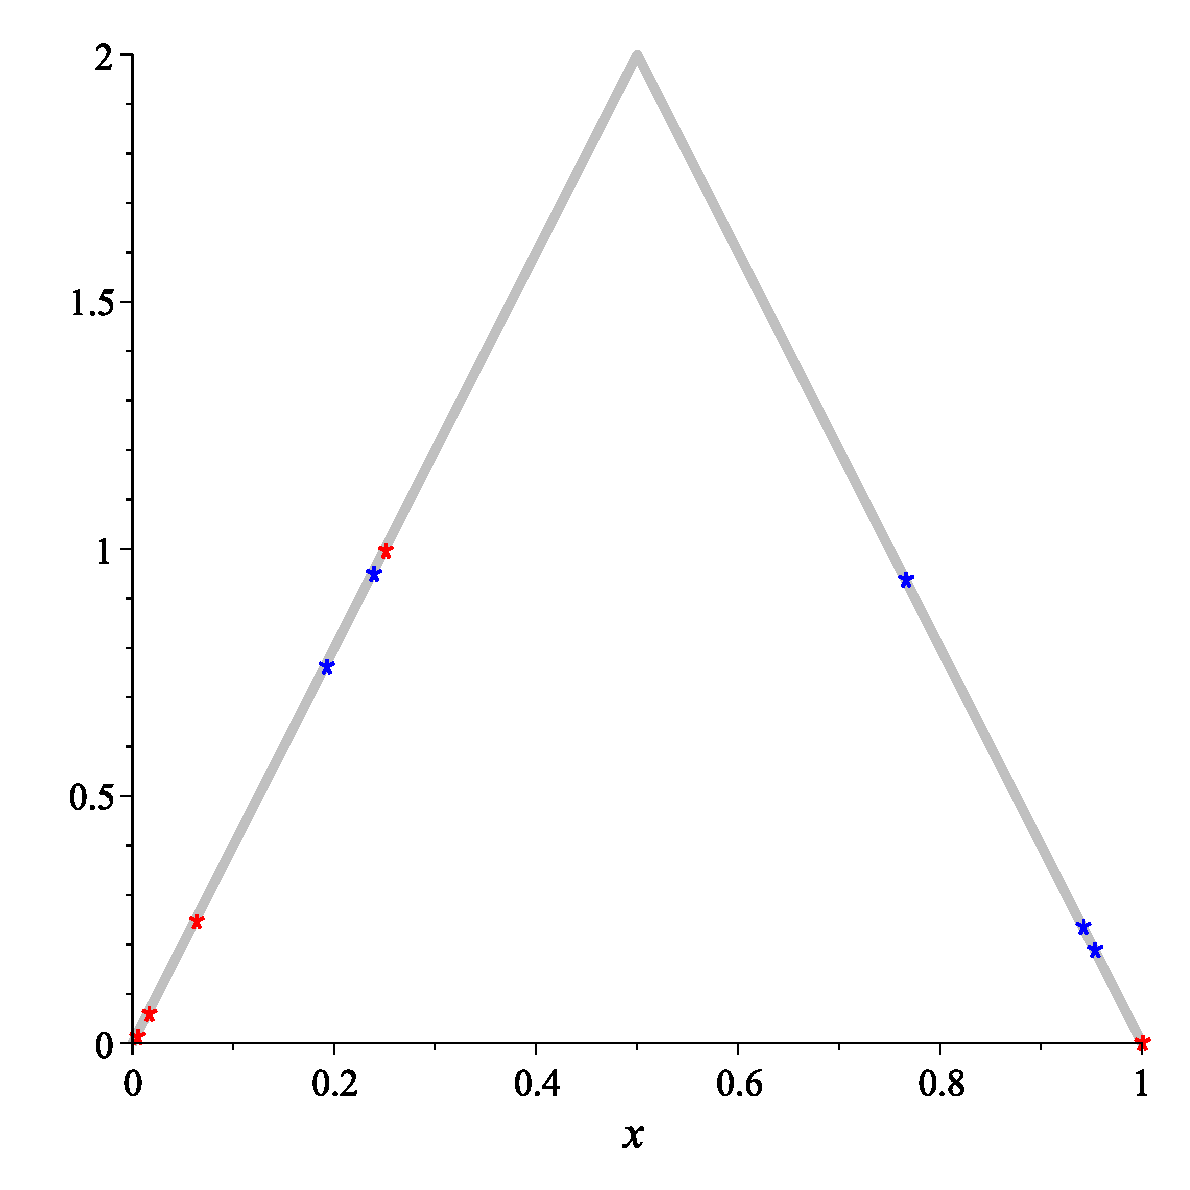
\includegraphics[scale=0.28]{Fig3a}
\hspace{1cm}
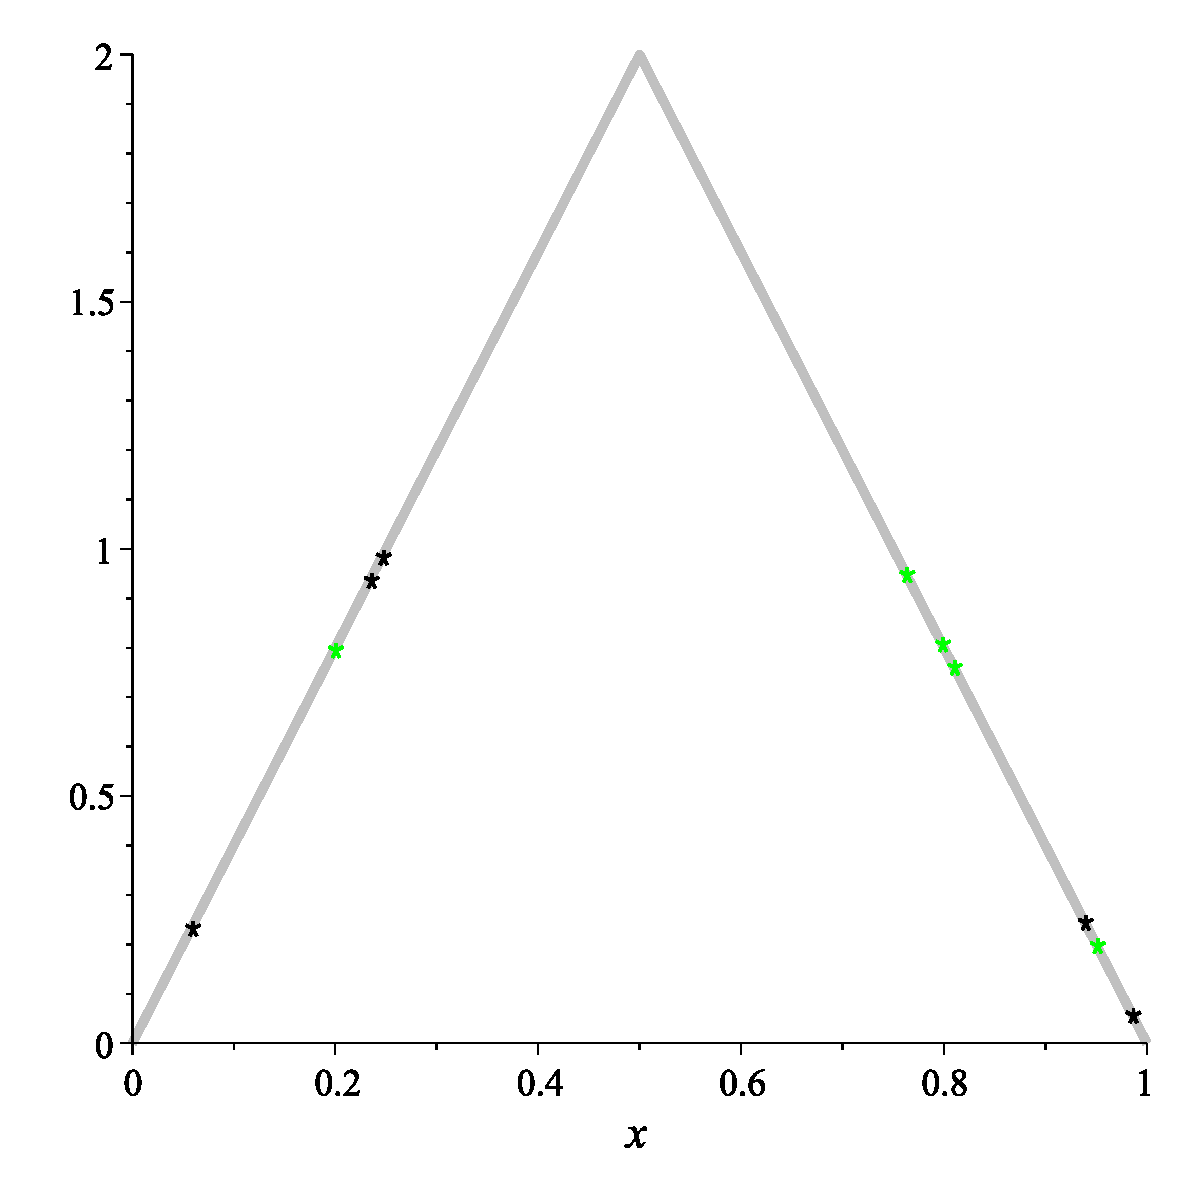
\includegraphics[scale=0.28]{Fig3b}
\caption{Cyclic points of 5-cycles of the tent map in the case of positive (red and blue) and negative (green and black) multipliers} \label{f3}
\end{figure}

% Figure 4
\begin{figure}[h!]
\centering
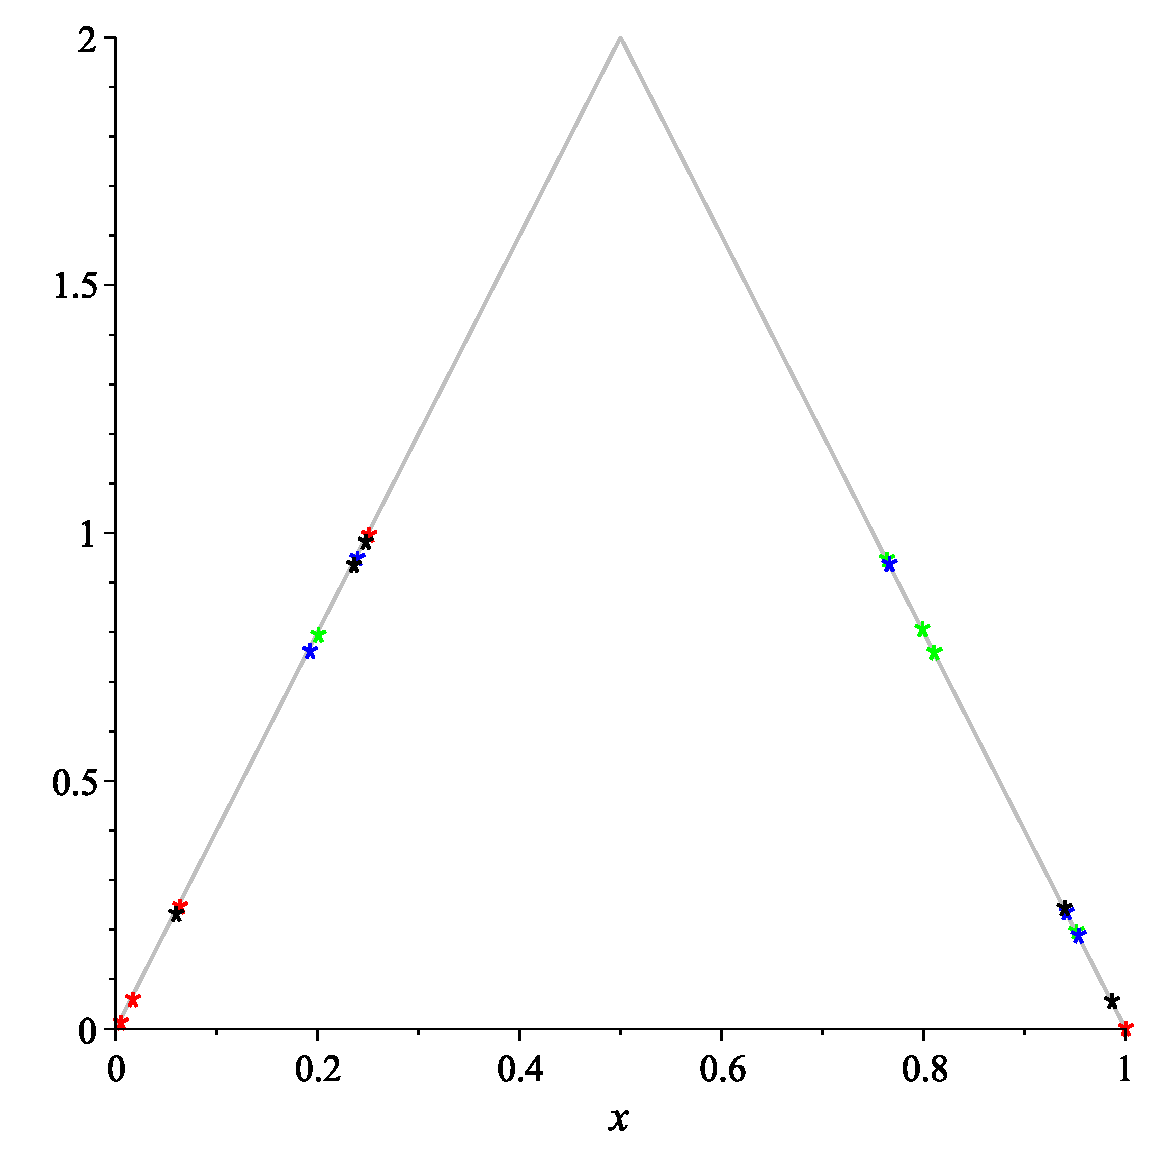
\includegraphics[scale=0.28]{Fig4}
\caption{Four sets of cyclic points of the tent map 5-cycles} \label{f4}
\end{figure}

% Figure 5
\begin{figure}[h!]
\centering
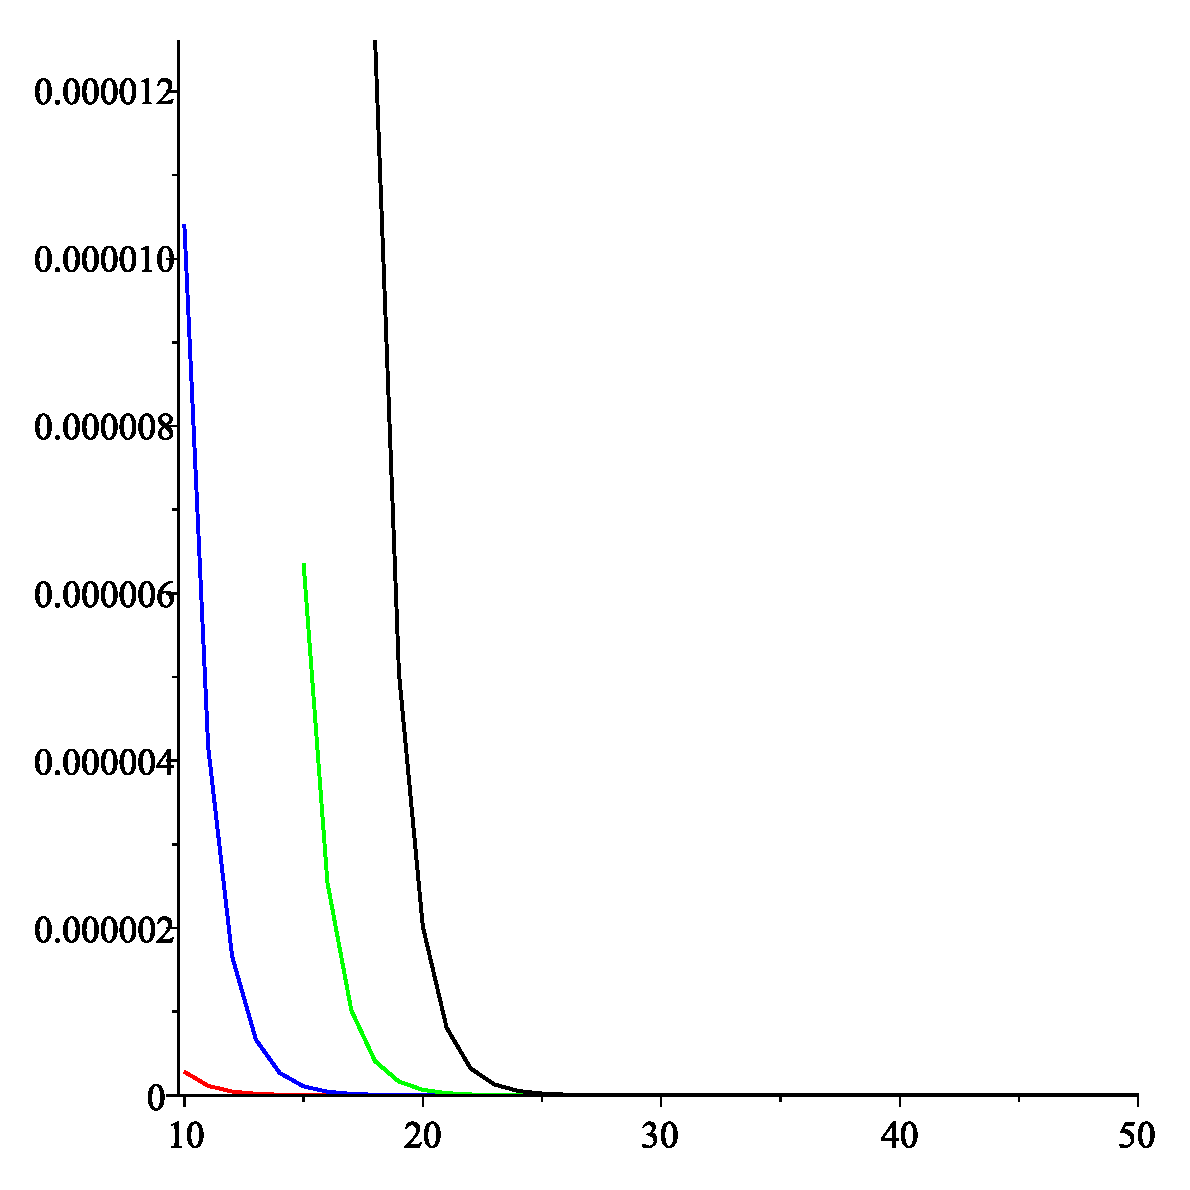
\includegraphics[scale=0.28]{Fig5a}
\hspace{1cm}
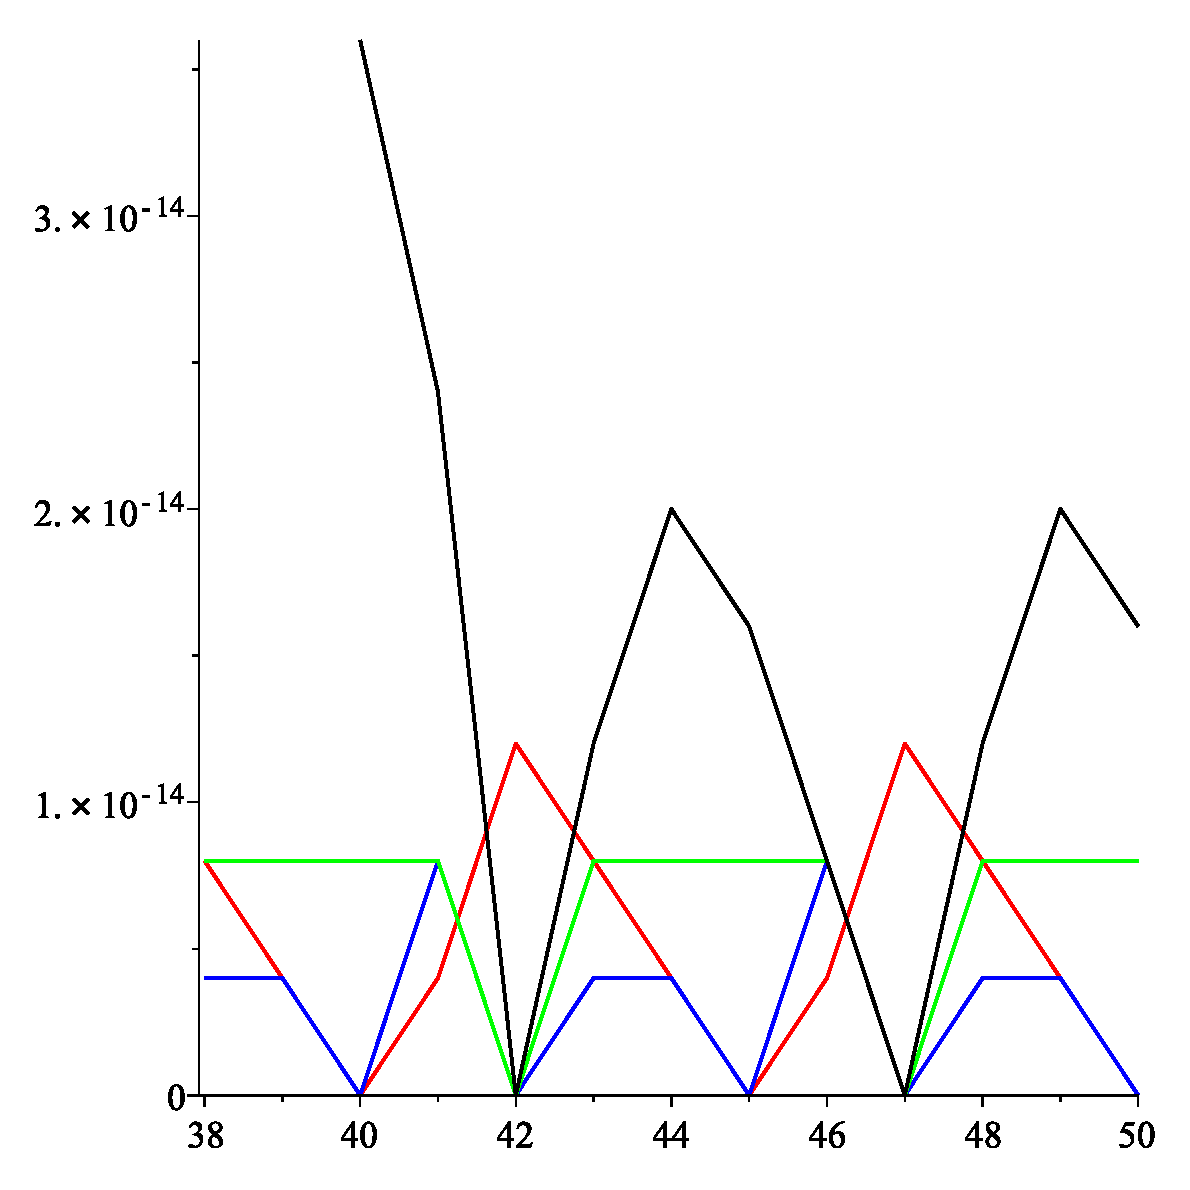
\includegraphics[scale=0.28]{Fig5b}
\caption{Residual for the periodic points of 5-cycles at $n=10..50$ and $n=38..50$} \label{f5}
\end{figure}

% Figure 6
\begin{figure}[h!]
\centering
\includegraphics[scale=0.28]{Fig6}
\caption{Four sets of cyclic points of the tent map 100-cycles} \label{f6}
\end{figure}

% Figure 7
\begin{figure}[h!]
\centering
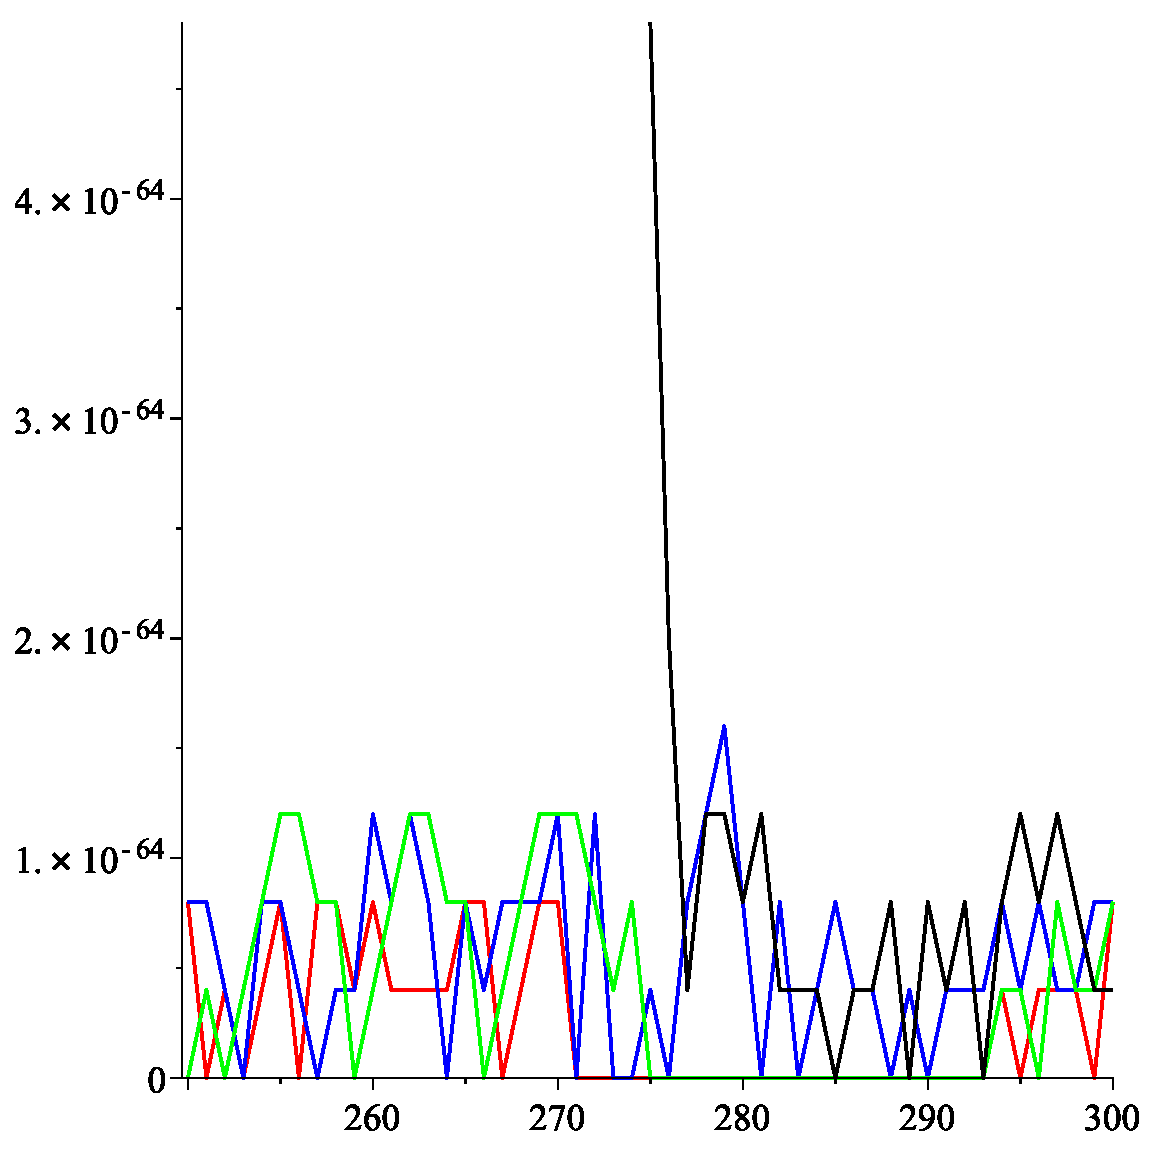
\includegraphics[scale=0.28]{Fig7}
\caption{Residual for the periodic points of 100-cycles at $n=250..300$} \label{f7}
\end{figure}

%_________________________________________________________________________________
\section{\centering{Graphical study of the control system map}}

Equation~(\ref{eq}) has two equilibria $\eta = 0$ and $\eta = \frac{H}{H+1}$, moreover, both are unstable; 
their multipliers are $H$ and $-H$ respectively. Consider the equation~(\ref{ceq})
$$
x_{n+1} = f \left( \vartheta x_n + (1 - \vartheta)f(x_n) \right)
$$
for different values of $\vartheta \in \left[0,\, \frac{H^T + \frac{1}{H}}{H^T-1}\right].$ For definiteness, set $H=3.$
Then $\left[0,\, \frac{H^T + \frac{1}{H}}{H^T-1}\right] = \left[ 0,\,\frac53\right].$ To stabilize the equilibrium $\eta=0,$
we need to choose the control parameter from the interval $\left(\frac43,\,\frac53\right),$ and with an increase 
in the control parameter from $\frac43$ to $\frac53$, the multiplier of this equilibrium decreases from $1$ to $-1$ 
(when $\vartheta=\frac32,$ the multiplier equals zero). The graphs of the function 
$y = f \left( \vartheta x + (1 - \vartheta)f(x) \right)$ for different values of $\vartheta$ are shown in Fig.~\ref{f8}.

% Figure 8
\begin{figure}[h!]
\centering
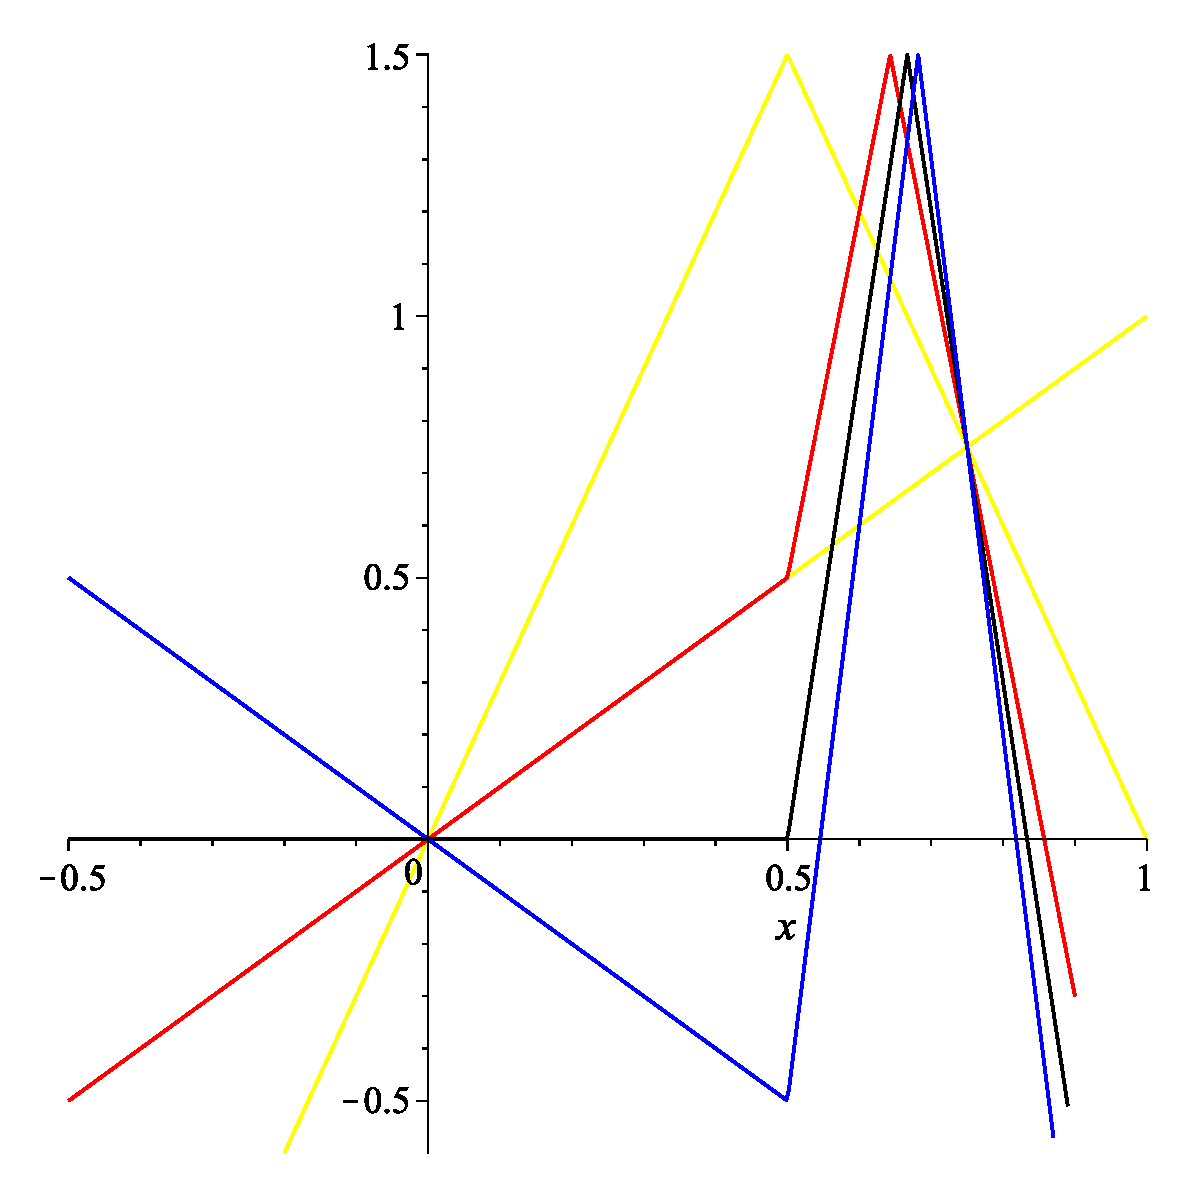
\includegraphics[scale=0.28]{Fig8}
\caption{Graphs of the function $y = f \left( \vartheta x + (1 - \vartheta)f(x) \right)$ at $\vartheta=\frac43$ (red);
at $\vartheta=\frac32$ (black); at $\vartheta=\frac53$ (blue); graphs of the functions $y=x$ and $y=f(x)$ 
are marked in yellow} \label{f8}
\end{figure}

The equilibrium $\eta=\frac34$ will be a locally asymptotically stable equilibrium of equation~(\ref{ceq}) at 
$\vartheta \in \left(\frac23,\,\frac56\right).$ As the control parameter increases, the multiplier of this equilibrium 
decreases from $1$ to $-1.$ When $\vartheta=\frac34,$ the multiplier equals zero. The graphs of the function 
$y = f \left( \vartheta x + (1 - \vartheta)f(x) \right)$ for different values of $\vartheta$ are depicted in Fig.~\ref{f9}. 

% Figure 9
\begin{figure}[h!]
\centering
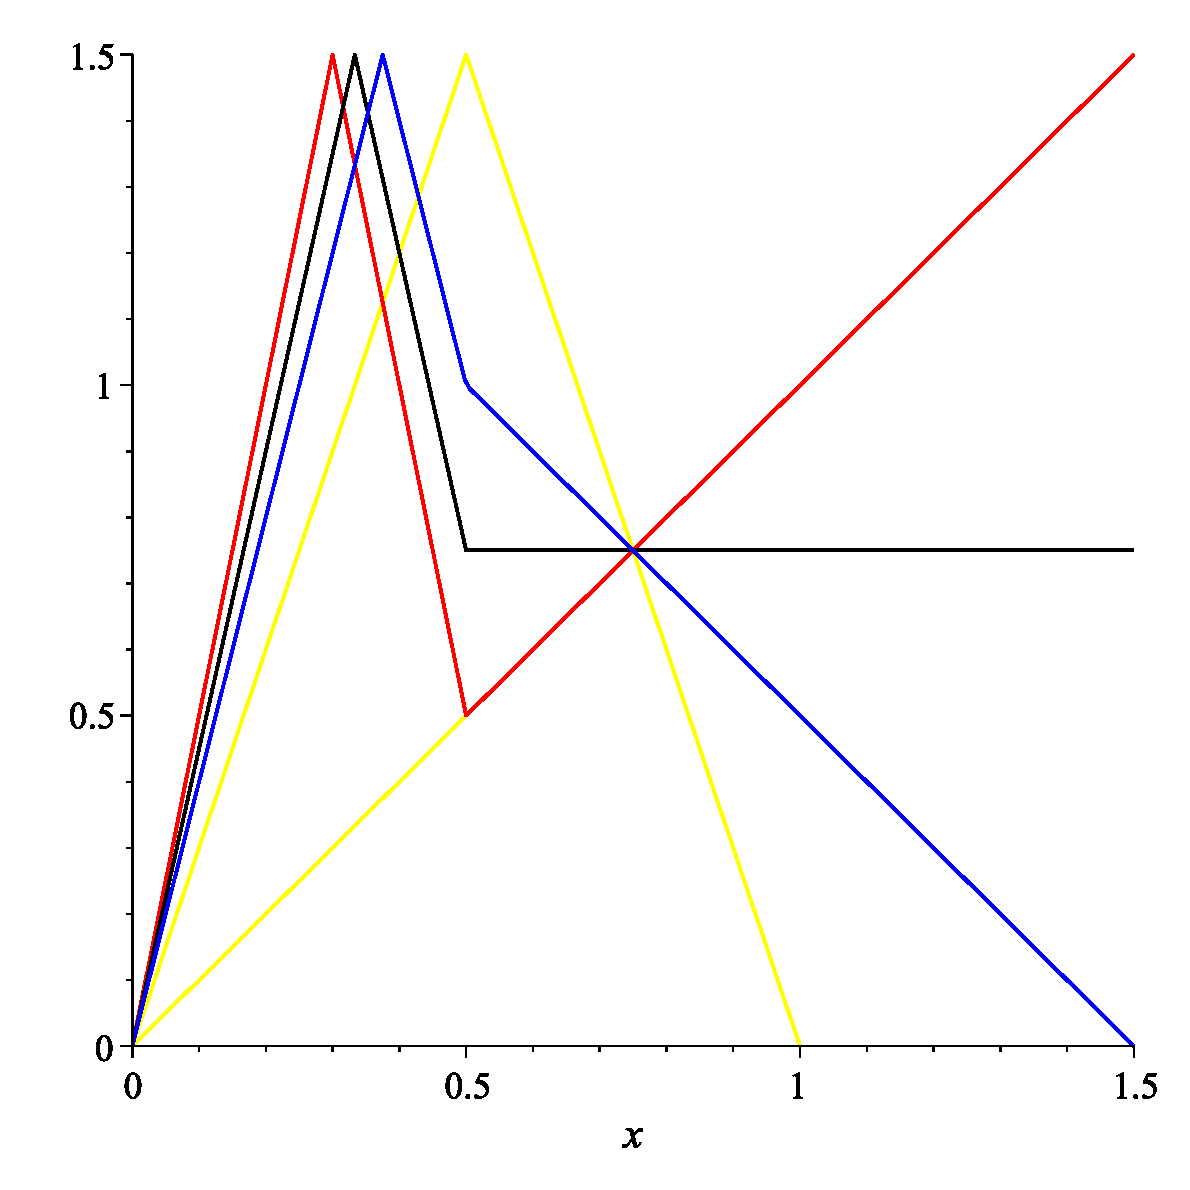
\includegraphics[scale=0.28]{Fig9}
\caption{Graphs of the function $y = f \left( \vartheta x + (1 - \vartheta)f(x) \right)$ at $\vartheta=\frac23$ (red);
at $\vartheta=\frac34$ (black); at $\vartheta=\frac56$ (blue); graphs of the functions $y=x$ and $y=f(x)$ 
are marked in yellow} \label{f9}
\end{figure}

If we represent the Lamerey diagram on the graphs of Fig.~\ref{f8}, then we can observe that for any initial value $x_0$ 
and $\vartheta \in \left(\frac43,\,\frac53\right),$ the corresponding solution of equation~(\ref{ceq}) will tend to zero. 
Analogously, Fig.~\ref{f9} can illustrate that the segment $\left[ 0,\,\frac32\right],$ under the mapping  
$y = f \left( \vartheta x + (1 - \vartheta)f(x) \right)$ (and at $\vartheta \in \left(\frac23,\,\frac56\right)$) goes into itself.
Moreover, for any $x_0 \in \left(0,\,\frac32\right),$ the solution tends to the equilibrium $\eta = \frac34.$ These facts are 
not difficult to obtain analytically as well.

Let $T=2.$ Equation~(\ref{eq}) has the only 2-cycle, and its multiplier is negative. The corresponding equation~(\ref{ceq}) 
takes the form $x_{n+1} = f \left( \vartheta x_n + (1 - \vartheta)f^{(2)}(_nx) \right).$ Consider the graphs of the functions 
$y=F(x),$ $y=F^{(2)}(x),$ where $F(x) = f \left( \vartheta x + (1 - \vartheta)f^{(2)}(x) \right)$ at 
$\vartheta = \frac{H^T}{H^T-1} = \frac98$ and $\vartheta = \frac{H^T}{H^T+1} = \frac{9}{10}$ 
(Fig.~\ref{f10}, Fig.~\ref{f11} -- a), b)).

% Figure 10
\begin{figure}[h!]
\centering
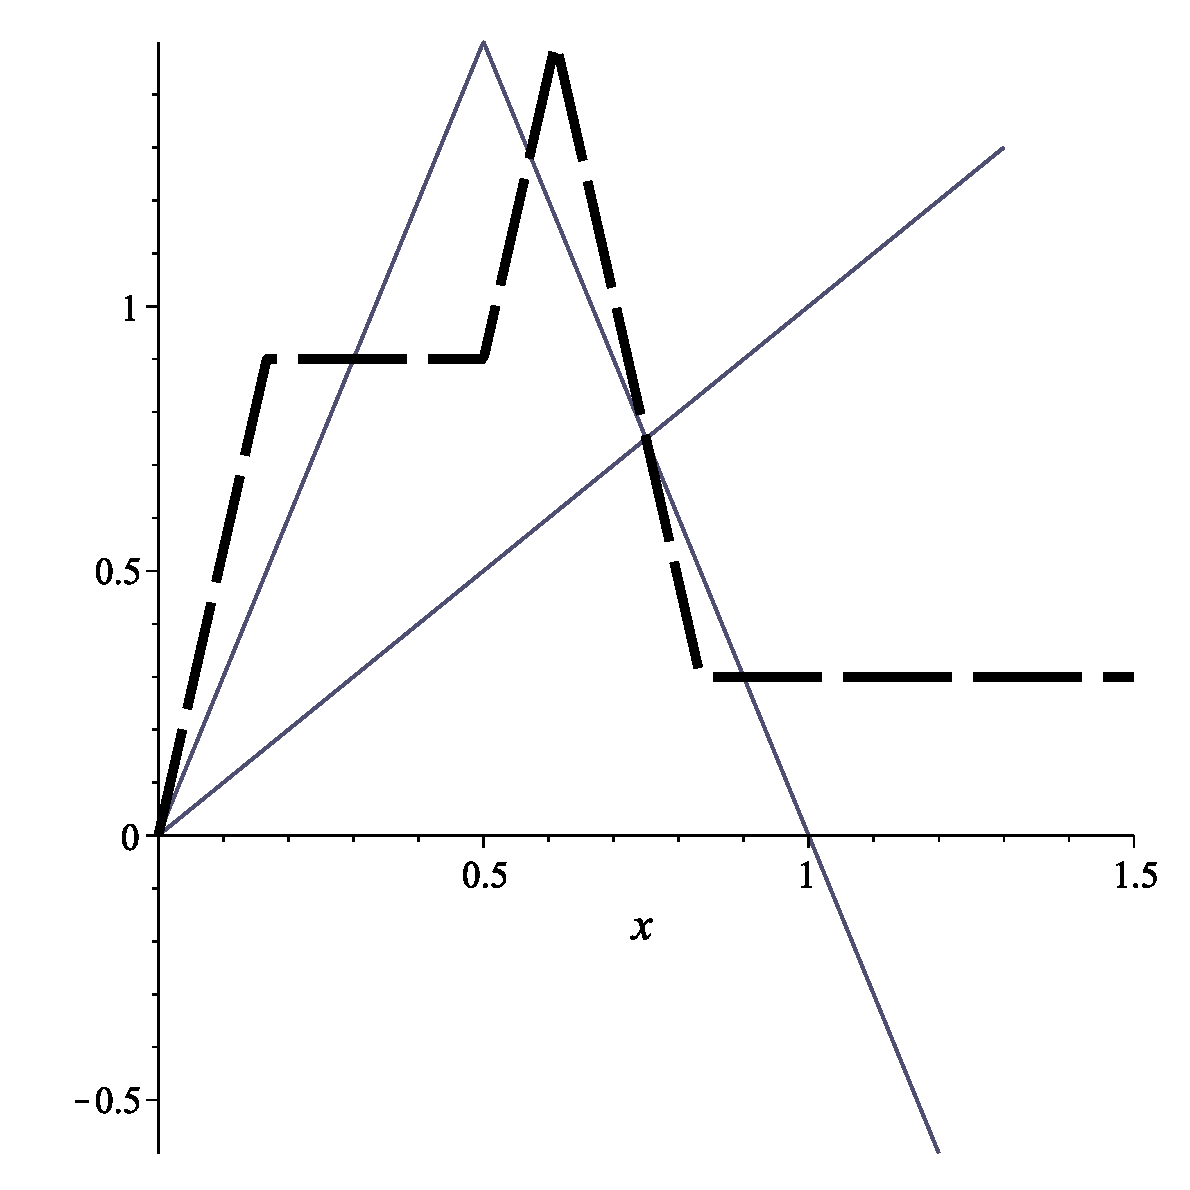
\includegraphics[scale=0.28]{Fig10}
\caption{Graphs of the function $y = F(x)$ at $\vartheta=\frac{9}{10}$ (black dashed line); 
$y=x$ and $y=f(x)$ (yellow)} \label{f10}
\end{figure}

% Figure 11
\begin{figure}[h!]
\begin{minipage}[h]{0.45\linewidth}
\center{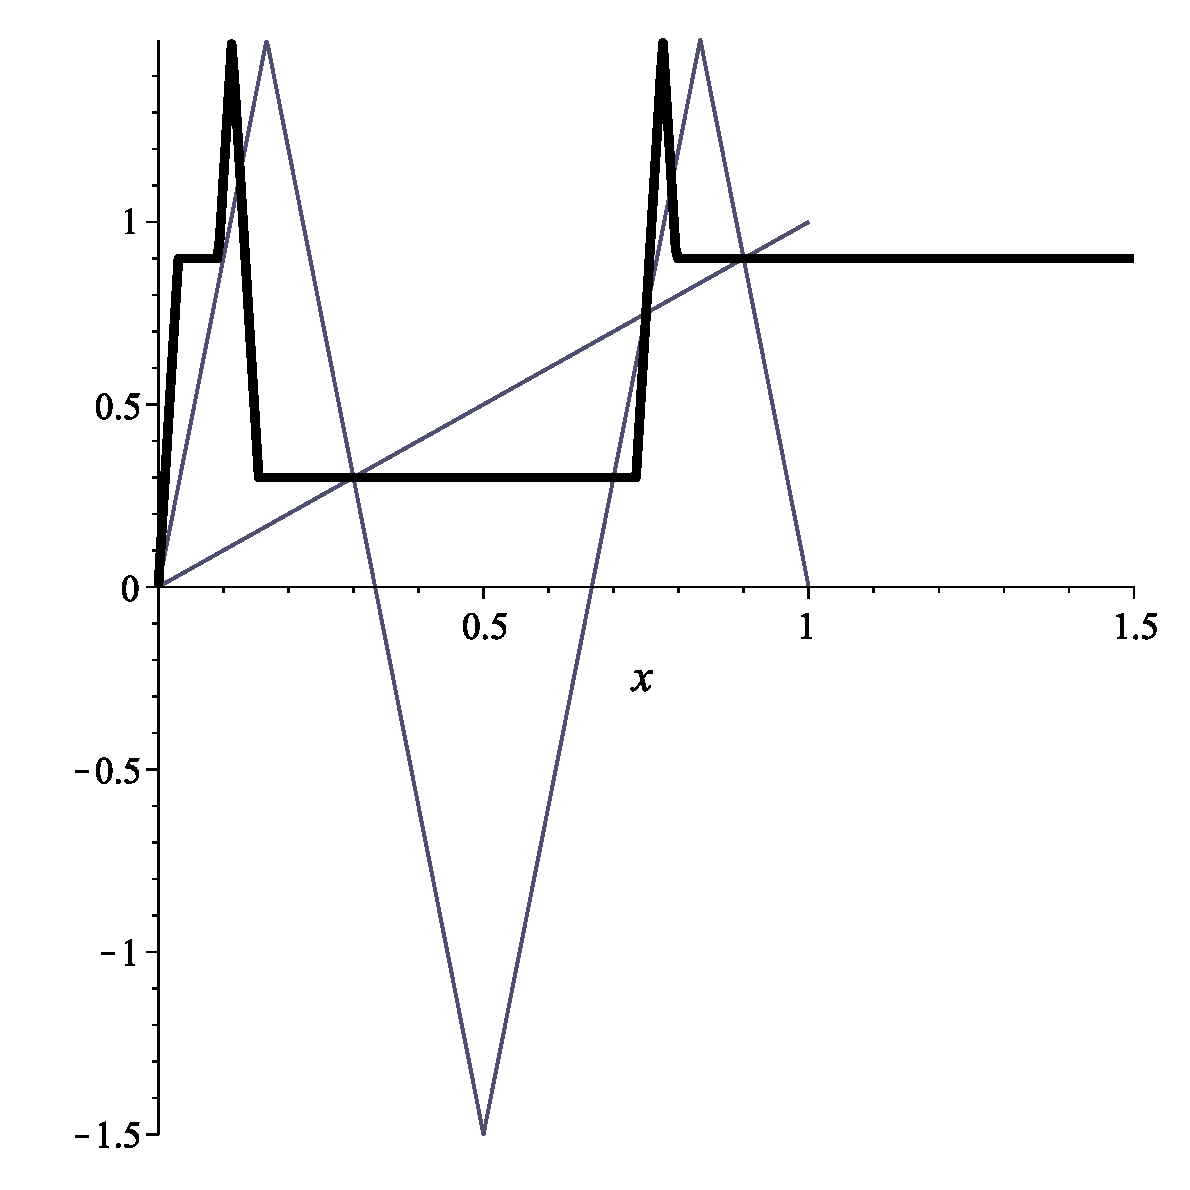
\includegraphics[scale=0.28]{Fig11a} \\ a)}
\end{minipage}
\hspace{1cm}
\begin{minipage}[h]{0.45\linewidth}
\center{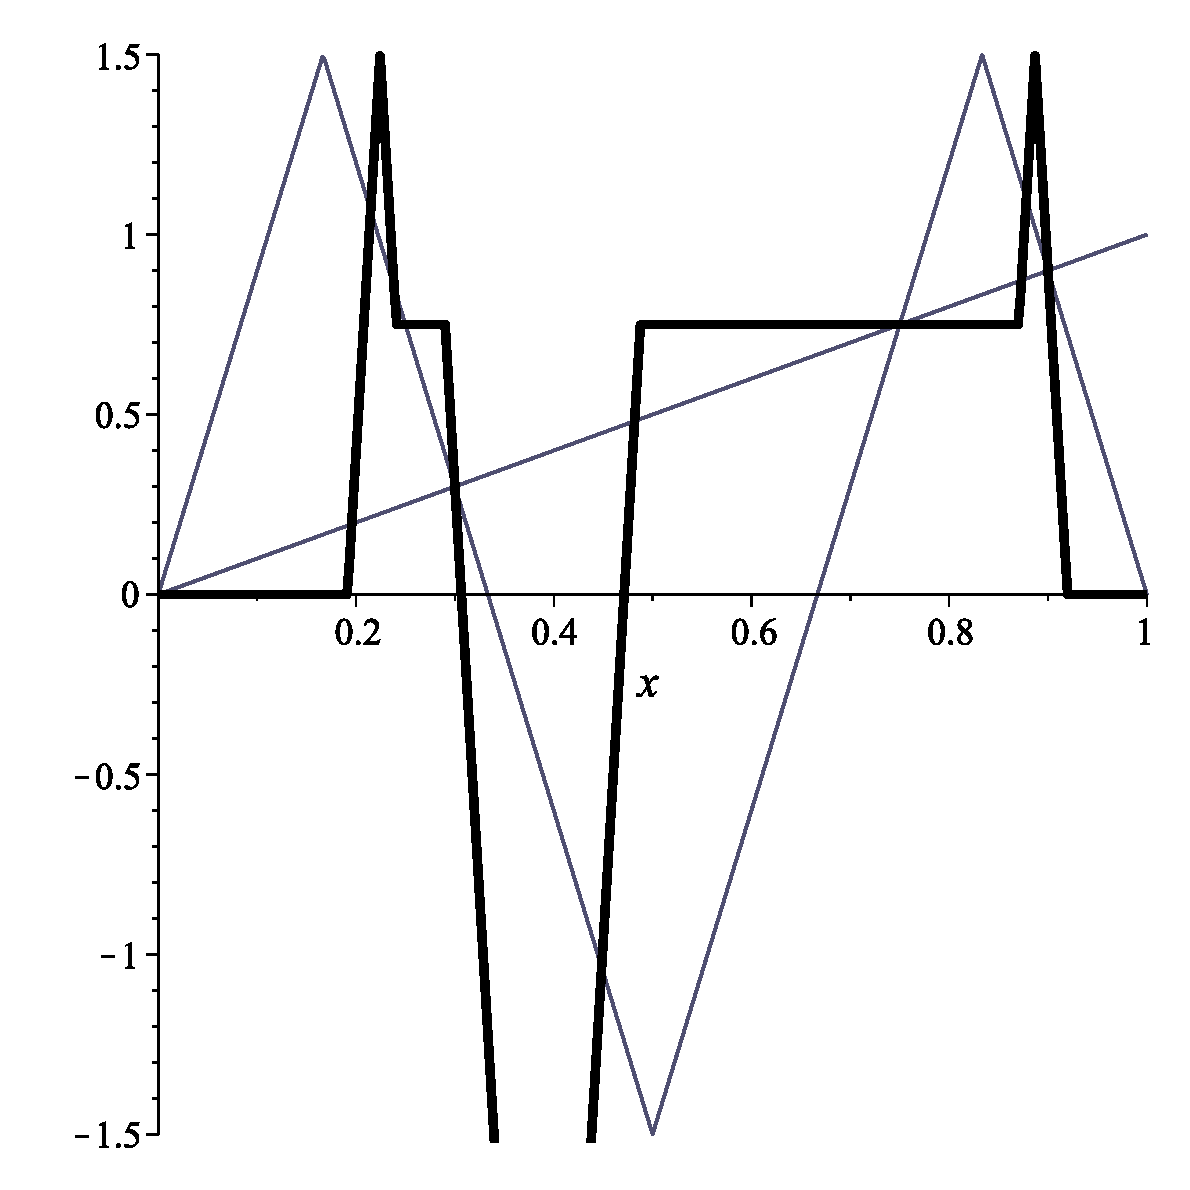
\includegraphics[scale=0.28]{Fig11b} \\ b)}
\end{minipage}
\caption{Graphs of the function $y = F^{(2)}(x)$ at $\vartheta=\frac{9}{10}$ (black); at $\vartheta=\frac{9}{8}$ (blue);
graphs of the functions $y=x$ and $y=f^{(2)}(x)$ are marked in yellow} \label{f11}
\end{figure}

From Fig.~\ref{f10}, we can see that the set $\left[ 0,\,\frac32\right]$ is invariant under the mapping $y=F(x),$ in Fig.~\ref{f11}-a) --
that the 2-cycle of equation~(\ref{ceq}) becomes locally asymptotically stable with the multiplier equal to zero. From 
Fig.~\ref{f11}-b), it is seen that the 2-cycle of equation~(\ref{ceq}) is unstable, but both equilibria are locally asymptotically stable 
(with zero multipliers). An explanation of this fact will be given in the next section.

Consider the global behavior of solutions of equation~(\ref{ceq}) at $\vartheta = \frac{H^T}{H^T+1}.$ The function 
$$
\zeta (x) = \frac{H^T}{H^T+1} x + \frac{1}{H^T+1}	f^{(T)}(x)
$$
does not decrease on $(-\infty;\infty).$ Indeed, 
$
\zeta'(x) = \frac{H^T \pm H^T}{H^T+1} =
\left\{\begin{array}{ll}
0,\,x\in \Sigma, \\
\frac{2 H^T}{H^T+1},\,x \notin\Sigma,
\end{array}\right.
$
where $\Sigma$ is the set on which the function $f^{(T)}(x)$ decreases. Note that the sets of increasing of the functions $f^{(T)}(x)$ 
and $\zeta (x)$ coincide. In particular, the function $\zeta (x)$ increases when 
$x \in \left( \frac12,\, 1-\frac{1}{H}+\frac{1}{2 H^{T-1}} \right)$ from $-\frac12 H^{T-1} (H-1)$ to $\frac{H}{2}.$ The point 
$\left( \frac12,\, -\frac12 H^{T-1} (H-1) \right)$ is the only point of the global minimum of the function $f^{(T)}(x).$ Fig.~\ref{f12} 
presents the graphs of the functions $f^{(T)}(x)$ and $\zeta (x)$ at $H=3,$ $T=3.$

% Figure 12
\begin{figure}[h!]
\centering
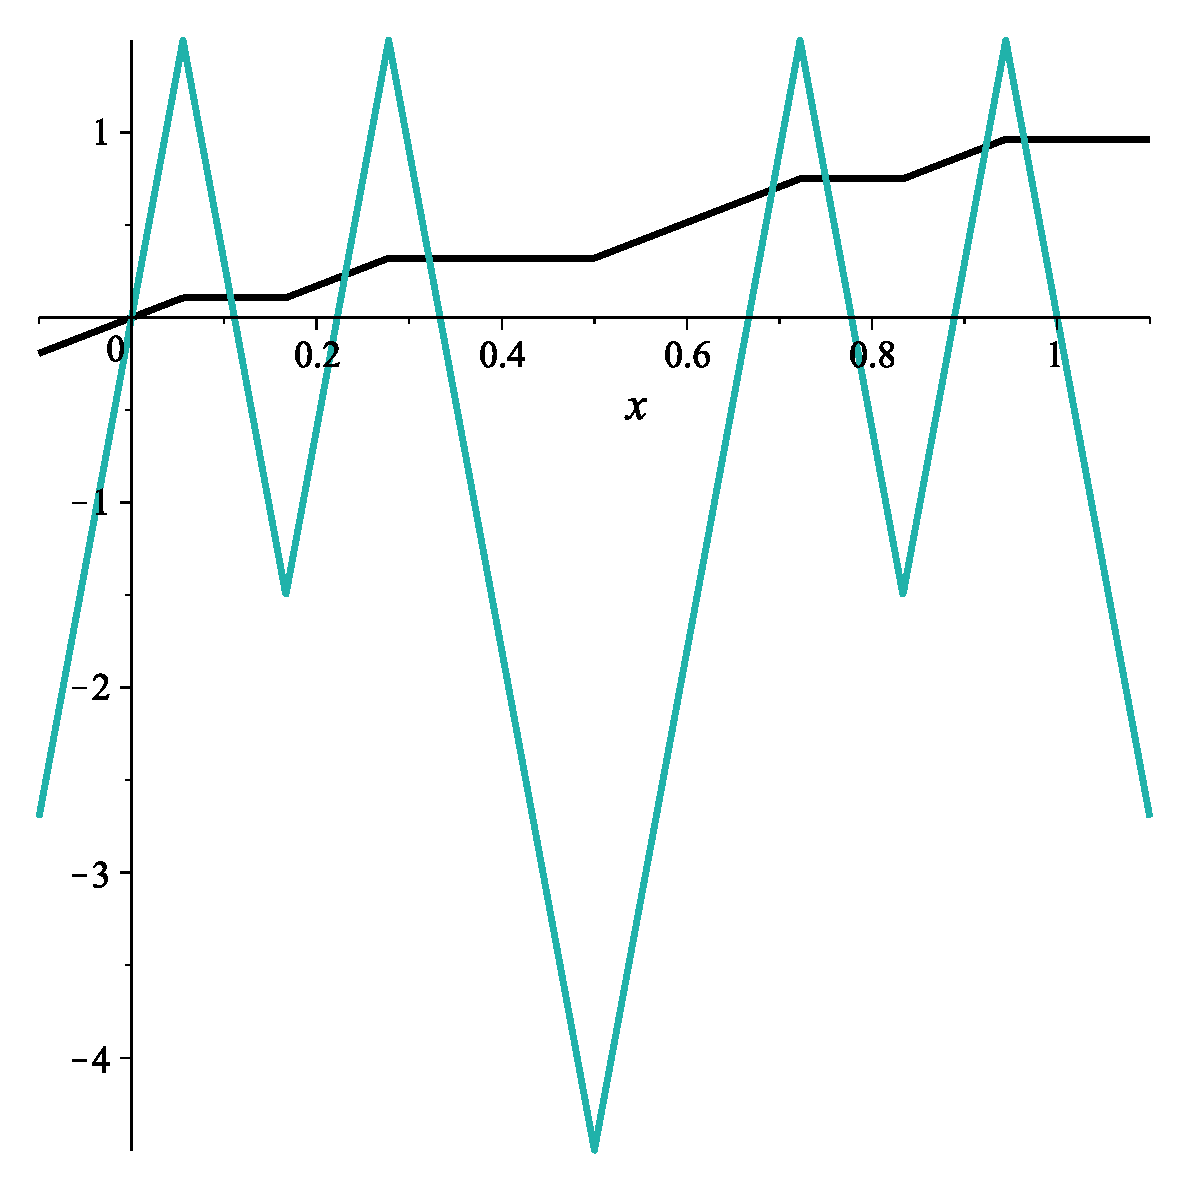
\includegraphics[scale=0.28]{Fig12}
\caption{Graphs of the functions $f^{(T)}(x)$ (blue) and $\zeta (x)$ (black) at $H=3,$ $T=3.$} \label{f12}
\end{figure}

Let $x \in \left( \frac12,\, 1-\frac{1}{H}+\frac{1}{2 H^{T-1}}  \right),$ $T>1.$ Denote $x = 1 - \frac{1}{H} + \frac{\alpha}{H^T}.$
Then $\alpha \in \left( -\frac12 H^{T-1} (H-2),\, \frac{H}{2} \right).$ Compute $f^{(T)}(x):$ $f(x) = 1 - \frac{\alpha}{H^{T-1}}>\frac12,$
$f^{(2)}(x) = \frac{\alpha}{H^{T-2}}<\frac12,$ \ldots , $f^{(T)}(x)=\alpha.$ This implies that the equation 
$\frac{H^T}{H^T+1} \left( 1-\frac{1}{H}+\frac{\alpha}{H^T} \right) + \frac{1}{H^T+1} \alpha = \frac12$ 
has only one root on $\left( -\frac12 H^{T-1} (H-2),\, \frac{H}{2} \right):$ $\widehat{\alpha} = \frac14 - \frac14 H^T + \frac12 H^{T-1}.$
Since $\zeta \left(\frac12\right) = \frac{H^{T-1}}{H^T+1} < \frac12,$ 
$\zeta \left( 1 - \frac{1}{H} + \frac{1}{2 H^{T-1}} \right) = \frac{H^T - H^{T-1} + H}{H^T +1} > \frac12,$ then in the interval 
$x \in \left( \frac12,\, 1-\frac{1}{H}+\frac{1}{2 H^{T-1}}  \right)$ there is exactly one root of the equation $\zeta (x) = \frac12:$ 
$\hat{x} = 1 - \frac{1}{H} + \frac{\widehat{\alpha}}{H^T} = \frac34 - \frac{1}{2H} + \frac{1}{4 H^T}.$ This means that the function 
$F(x)=f(\zeta(x))$ does not decrease on the interval $\left[0,\,\hat{x}\right],$ does not increase on $\left[\hat{x},\,1\right],$
$F(\hat{x})=\frac{H}{2}$ and $F(x) = F \left( 1 - \frac{1}{2 H^{T-1}} \right) = \frac{H^T}{H^T + 1}$ when 
$\hat{x} \geq 1 - \frac{1}{2 H^{T-1}}.$ The graph of the function $F(x)$ at $H=3,$ $T=4$ is given in Fig.~\ref{f13}-a). Fig.~\ref{f13}-b) 
shows the corresponding graphs of the functions $F(x)$ and $\zeta(x).$

% Figure 13
\begin{figure}[h!]
\begin{minipage}[h]{0.45\linewidth}
\center{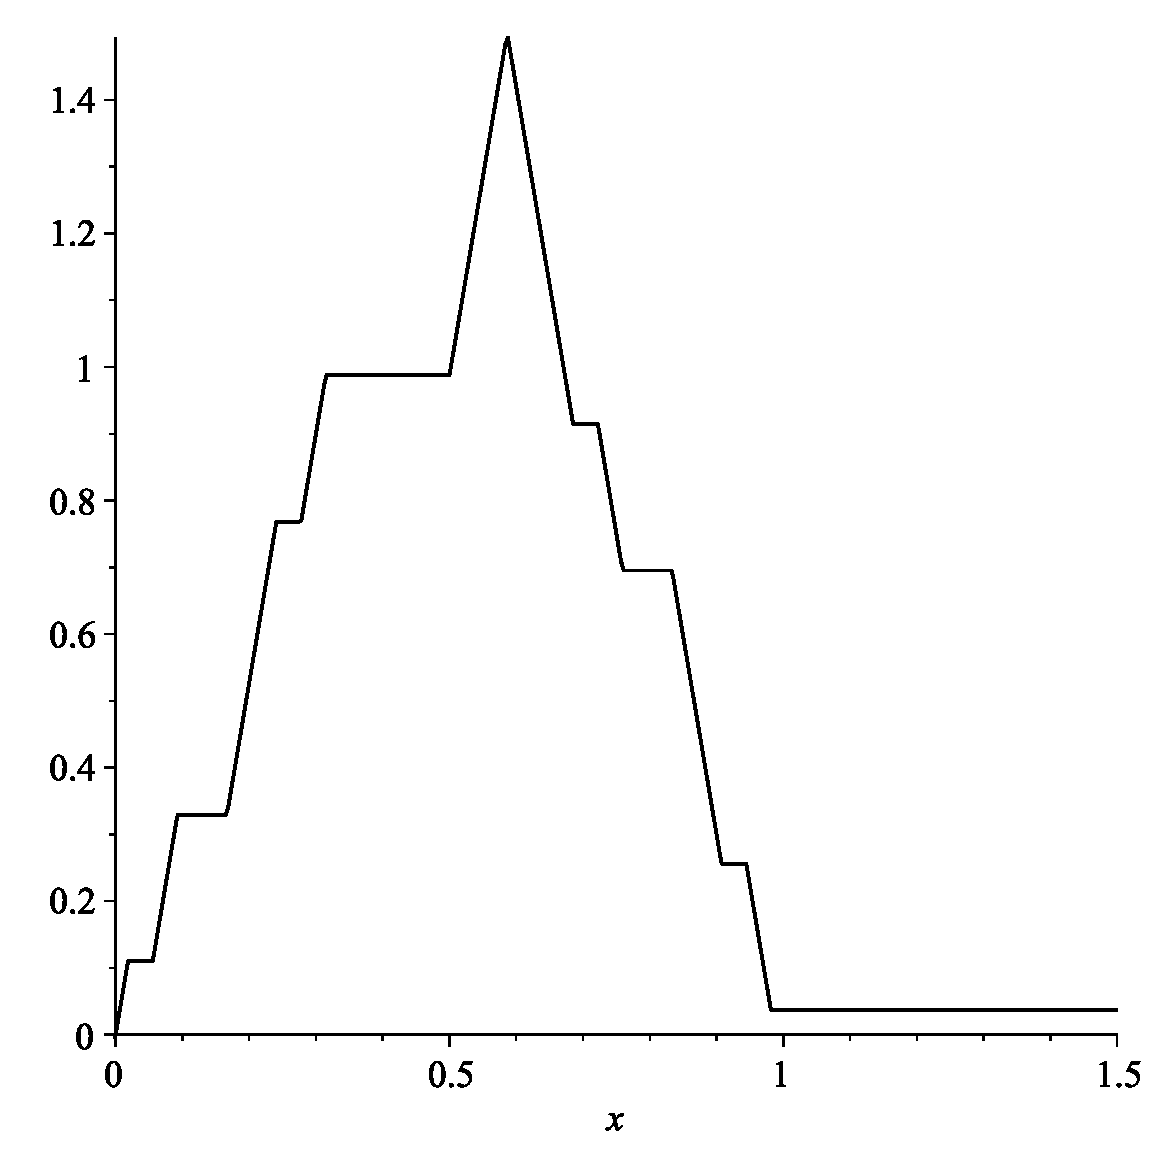
\includegraphics[scale=0.28]{Fig13a} \\ a)}
\end{minipage}
\hspace{1cm}
\begin{minipage}[h]{0.45\linewidth}
\center{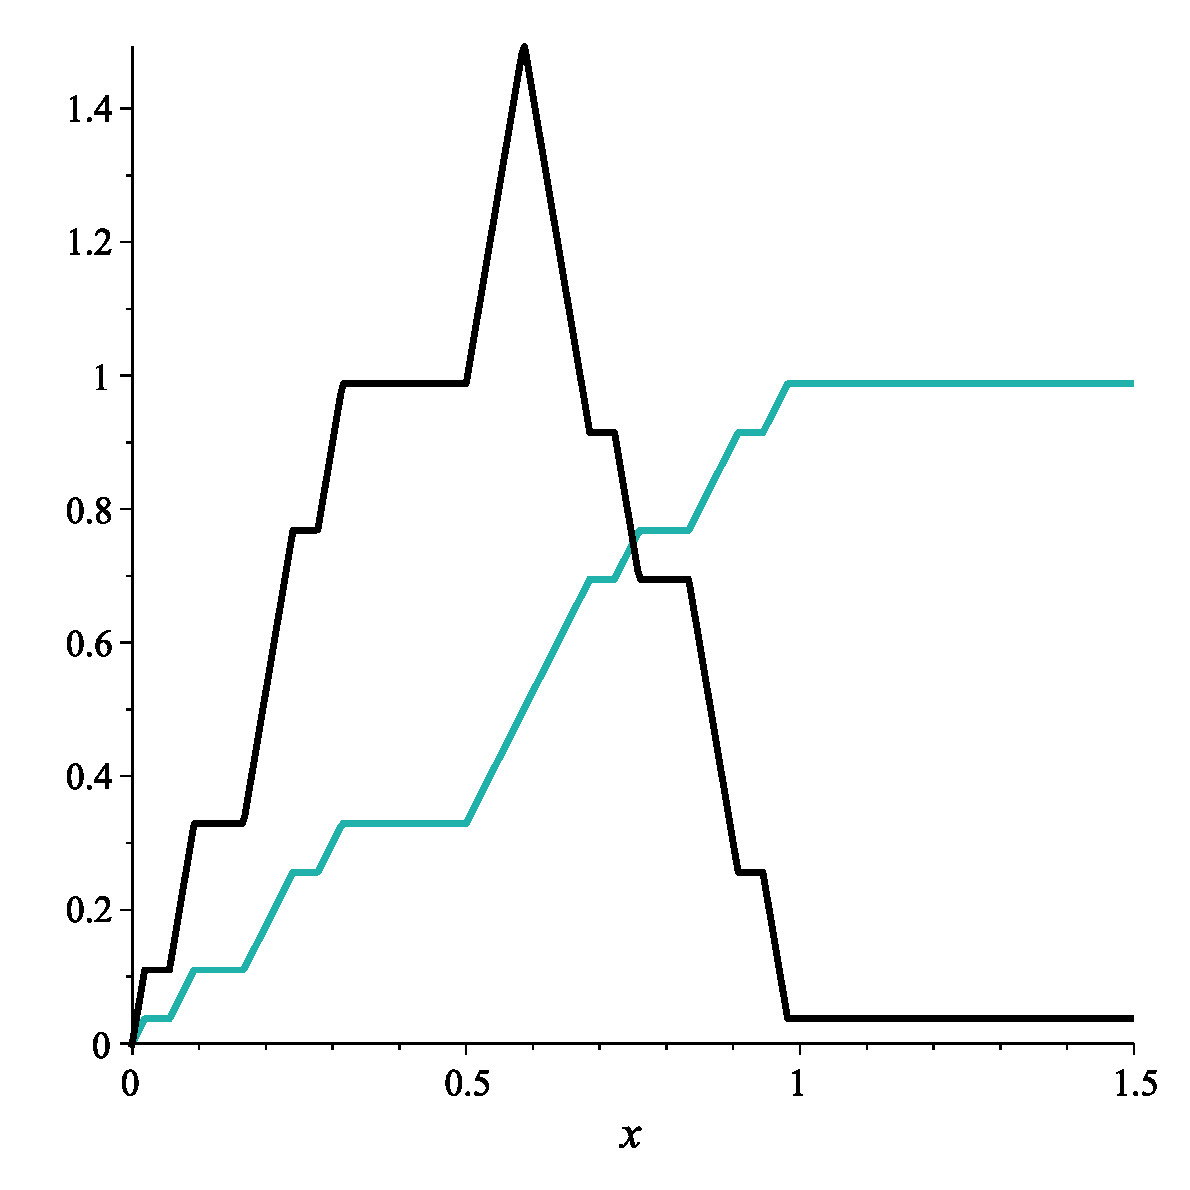
\includegraphics[scale=0.28]{Fig13b} \\ b)}
\end{minipage}
\caption{Graphs of the functions $F(x)$ (black) and $\zeta (x)$ (blue) at $H=3,$ $T=4.$} \label{f13}
\end{figure}

On the interval $[0,\,1],$ there exist $2^{T-1}$ disjoint intervals, where the function $F(x)$ is constant. This means that there exist $2^{T-1}$ 
periodic points, where $F'(x)=0.$ These points are $T$-periodic points of the map $f(x)$ with negative multipliers. Generally speaking, 
the proper period of these points may be less than $T,$ if $T$ is not a prime number. The question of stability of the so-called subcycles 
is considered in the next section. Equality to zero of the derivative means that the iterative process defined by equation~(\ref{ceq}) has 
ultrafast convergence to cyclic points. In particular, if $x_0 \geq \hat{x},$ then $x_1 = F(x_0) = \frac{H^T}{H^T + 1} > \frac12,$
$x_2 = F(x_1) = f(x_1) = \frac{H}{H^T + 1} < \frac12,$ \ldots , $x_T = F(x_{T-1}) = f(x_{T-1}) = \frac{H^{T-1}}{H^T + 1} < \frac12,$
$x_{T+1} = F(x_T) = f(x_T) = \frac{H^T}{H^T + 1} = x_1,$ i.e., $\left\{ x_1,\ldots,\,x_T\right\}$ is a cycle of equations~(\ref{eq}) and 
(\ref{ceq}). 

%_________________________________________________________________________________
\section{\centering{Subcycles}}

In equation~(\ref{eq}), for any natural $T \geq 1$ there exist $T$-cycles. Moreover, it is not difficult to estimate their number. The graph of the function 
$y = f^{(T)}(x)$ intersects with the graph of the function $y = x$ when $x\in[0,\,1]$ exactly $2^T$ times. Two points of intersection correspond to 
equilibria $x=0,$ $x = 1 - \frac{1}{H+1}$. This means that there are no more than $\frac{2^T - 2}{T}$ cycles of the length $T$ (excluding equilibria). 
If $T$ is a prime number, then there are exactly $\frac{2^T - 2}{T}$ cycles. The well-known result is easily obtained from this: for a prime number $T>2,$ 
the number $2^{T-1} - 1$ is divisible by $T.$ If $T = \prod\limits_{j=1}^{s} {\tau_{j}^{\rho_j}},$ where $\tau_1,\ldots,\,\tau_s$ are prime numbers, 
then there are exactly $\frac{2^T - \sum\limits_{j=1}^{s}{2^\frac{T}{\tau_j}} + \sum\limits_{\substack{i,\,j=1 \\ i<j}}^{s}{2^\frac{T}{\tau_i \tau_j}} + \ldots +
(-1)^s 2^\frac{T}{\tau_1 \cdot \ldots \cdot \tau_s}}{T}$ cycles of the length $T.$ The fact that the given fraction is an integer is a special case of 
Gauss's theorem.

Let $\tau$ be a factor of the number $T$ (if $T$ is a prime number, then we assume $\tau=1$). And let the $T$-cycle of equation~(\ref{ceq}) 
be locally asymptotically stable. \textit{The task} is: to find out in what cases $\tau$-cycles of the same equation will be locally asymptotically stable?

\begin{theorem}\label{t4}
Let condition~(\ref{inp}) be satisfied, i.e. $T$-cycles of equation~(\ref{eq}), for which the multipliers are positive, are locally asymptotically stable cycles 
of equation~(\ref{ceq}). Then all the $\tau$-cycles of equation~(\ref{eq}), for which the multipliers are positive, and all the $\tau$-cycles of 
equation~(\ref{eq}), for which the multipliers are negative and the number $\frac{T}{\tau}$ is even, are locally asymptotically stable cycles of 
equation~(\ref{ceq}).

Let condition~(\ref{inn}) be satisfied, i.e. $T$-cycles of equation~(\ref{eq}), for which the multipliers are negative, are locally asymptotically stable cycles 
of equation~(\ref{ceq}). Then all the $\tau$-cycles of equation~(\ref{eq}), for which the multipliers are negative and the number $\frac{T}{\tau}$ is odd, 
are locally asymptotically stable cycles of equation~(\ref{ceq}).
\end{theorem}

\begin{proof}
Let $\left\{\eta_1,\ldots,\,\eta_T\right\}$ be a $T$-cycle and $\left\{\widehat{\eta}_1,\ldots,\,\widehat{\eta}_\tau\right\}$ be a $\tau$-cycle of 
equation~(\ref{eq}). Let $\mu_T = f'(\eta_T)\cdot\ldots\cdot f'(\eta_1),$ $\mu_\tau = f'(\widehat{\eta}_\tau)\cdot\ldots\cdot f'(\widehat{\eta}_1)$ 
be the corresponding multipliers of these cycles. These cycles will also be the cycles of equation~(\ref{ceq}). We assume that the condition for local 
asymptotic stability of the $T$-cycle of equation~(\ref{ceq})
\begin{equation}\label{tc}
\left| \mu_T \left( \vartheta + (1 - \vartheta) \mu_T\right)^T\right| < 1 
\end{equation}
is satisfied. Let us find the multiplier of the $\tau$-cycle of equation~(\ref{ceq}). Let, as before, 
$F(x) = f \left( \vartheta x + (1-\vartheta) f^{(T)}(x)\right),$ and $p=\frac{T}{\tau}.$ Calculate
\begin{gather*}
F'(\widehat{\eta}_j) = f'(\widehat{\eta}_j) \left( \vartheta + (1-\vartheta) \left( f'(\widehat{\eta}_\tau)\cdot\ldots\cdot f'(\widehat{\eta}_1) \right)^p \right) = \\
= f'(\widehat{\eta}_j) \left( \vartheta + (1-\vartheta) (\mu_\tau)^p \right),\; j=1,\ldots,\,\tau.
\end{gather*}
Then the multiplier of the $\tau$-cycle of equation~(\ref{ceq}) equals 
$F'(\widehat{\eta}_\tau)\cdot\ldots\cdot F'(\widehat{\eta}_1) = \mu_\tau \left( \vartheta + (1-\vartheta) (\mu_\tau)^p \right)^\tau$, and, accordingly, 
the condition for local asymptotic stability of the $\tau$-cycle of equation~(\ref{ceq}) is:
\begin{equation}\label{tauc}
\left| \mu_\tau \left( \vartheta + (1 - \vartheta) (\mu_\tau)^p \right)^\tau \right| < 1 
\end{equation}

Since $\mu_T = \pm H^T,$ $\mu_\tau = \pm H^\tau,$ the following cases are possible:

\begin{enumerate}
\item[a)] $\mu_T<0,$ $\mu_\tau<0,$ then 
$\left\{\begin{array}{ll}
\mu_T = (\mu_\tau)^p,\, p \text{ is odd}, \\
\mu_T = -(\mu_\tau)^p,\, p \text{ is even},
\end{array}\right.$

\medskip
\item[b)] $\mu_T<0,$ $\mu_\tau>0,$ then $\mu_T = -(\mu_\tau)^p$ for any $p,$  

\medskip
\item[c)] $\mu_T>0,$ $\mu_\tau<0,$ then 
$\left\{\begin{array}{ll}
\mu_T = -(\mu_\tau)^p,\, p \text{ is odd}, \\
\mu_T = (\mu_\tau)^p,\, p \text{ is even},
\end{array}\right.$

\medskip
\item[d)] $\mu_T>0,$ $\mu_\tau>0,$ then $\mu_T = (\mu_\tau)^p$ for any $p.$  
\end{enumerate}

Inequality~(\ref{tc}) implies inequality~(\ref{tauc}) if and only if one of the conditions holds: $\mu_T<0,$ $\mu_\tau<0,$ $p$ is odd; 
$\mu_T>0,$ $\mu_\tau<0,$ $p$ is even; $\mu_T>0,$ $\mu_\tau>0$ for any $p.$ The first condition is possible for the parameters $\vartheta$ that satisfy 
inequalities~(\ref{inp}), the second and third conditions are so for the parameters $\vartheta$ that satisfy inequalities~(\ref{inn}), whence the conclusion 
of the Theorem follows.
\end{proof}

Consider again the example of stabilization of 5-cycles from Section~4, but take $x_0=0.001$ and $x_0=0.801$ as the initial points. Then, besides locally 
asymptotically stable 5-cycles, equilibria $\eta=0$ at $\vartheta = \frac{H^T + \frac{0.4}{H}}{H^T - 1}$ and $\eta=0.8$ at 
$\vartheta = \frac{H^T - \frac{0.4}{H}}{H^T + 1}$ will also be stable. The selected initial points get into the basins of attraction of the corresponding 
equilibria. Periodic and fixed points are shown in Fig.~\ref{f14} (the colors remain the same).

% Figure 14
\begin{figure}[h!]
\centering
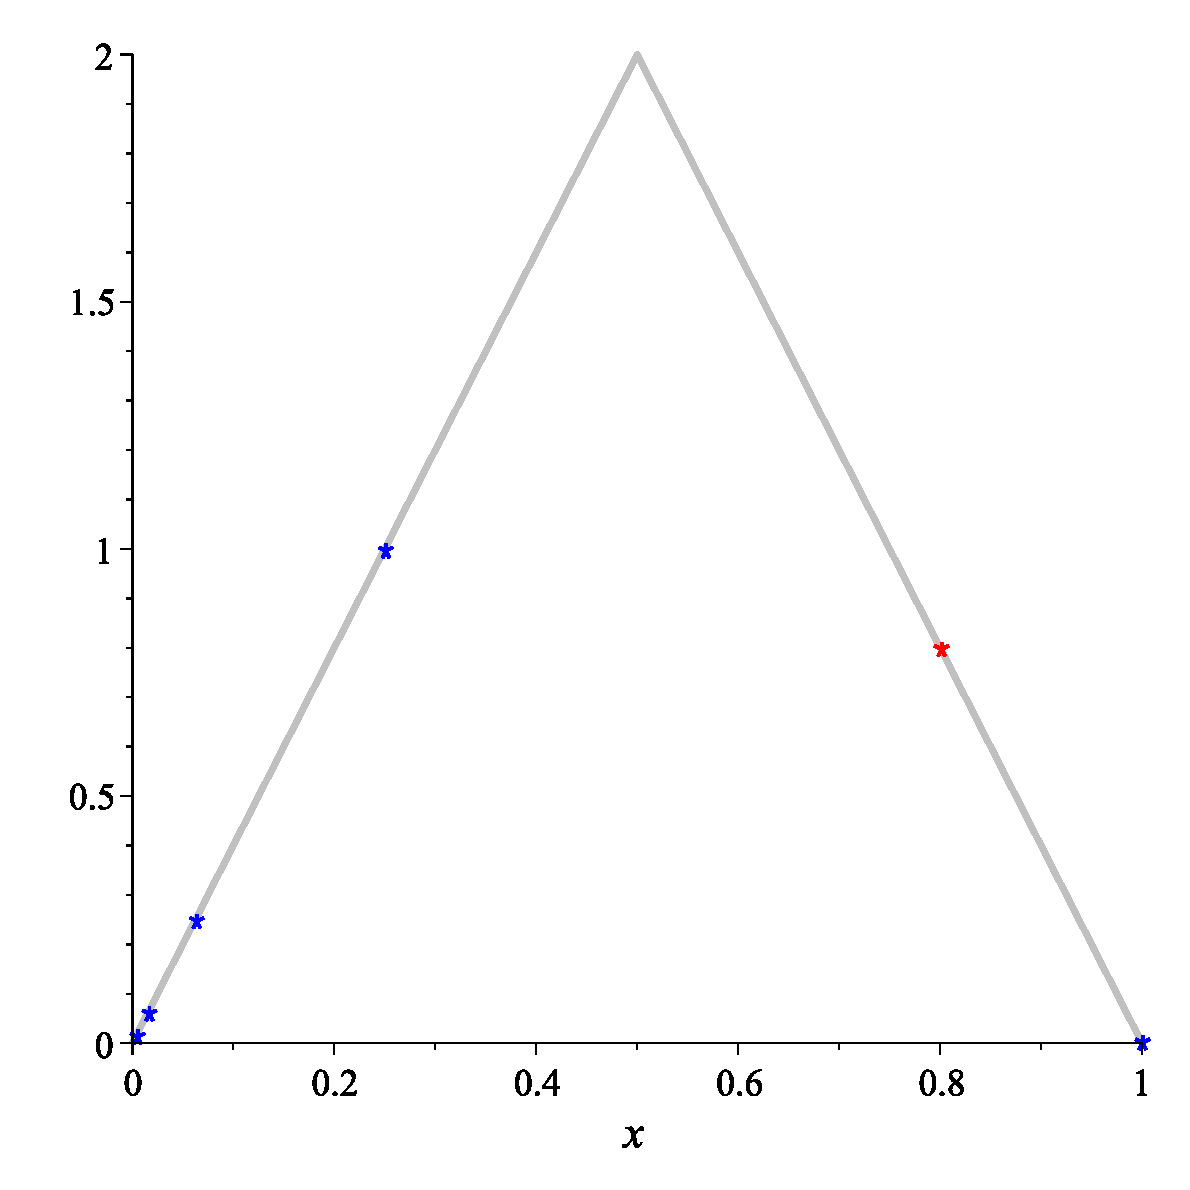
\includegraphics[scale=0.28]{Fig14a}
\hspace{1cm}
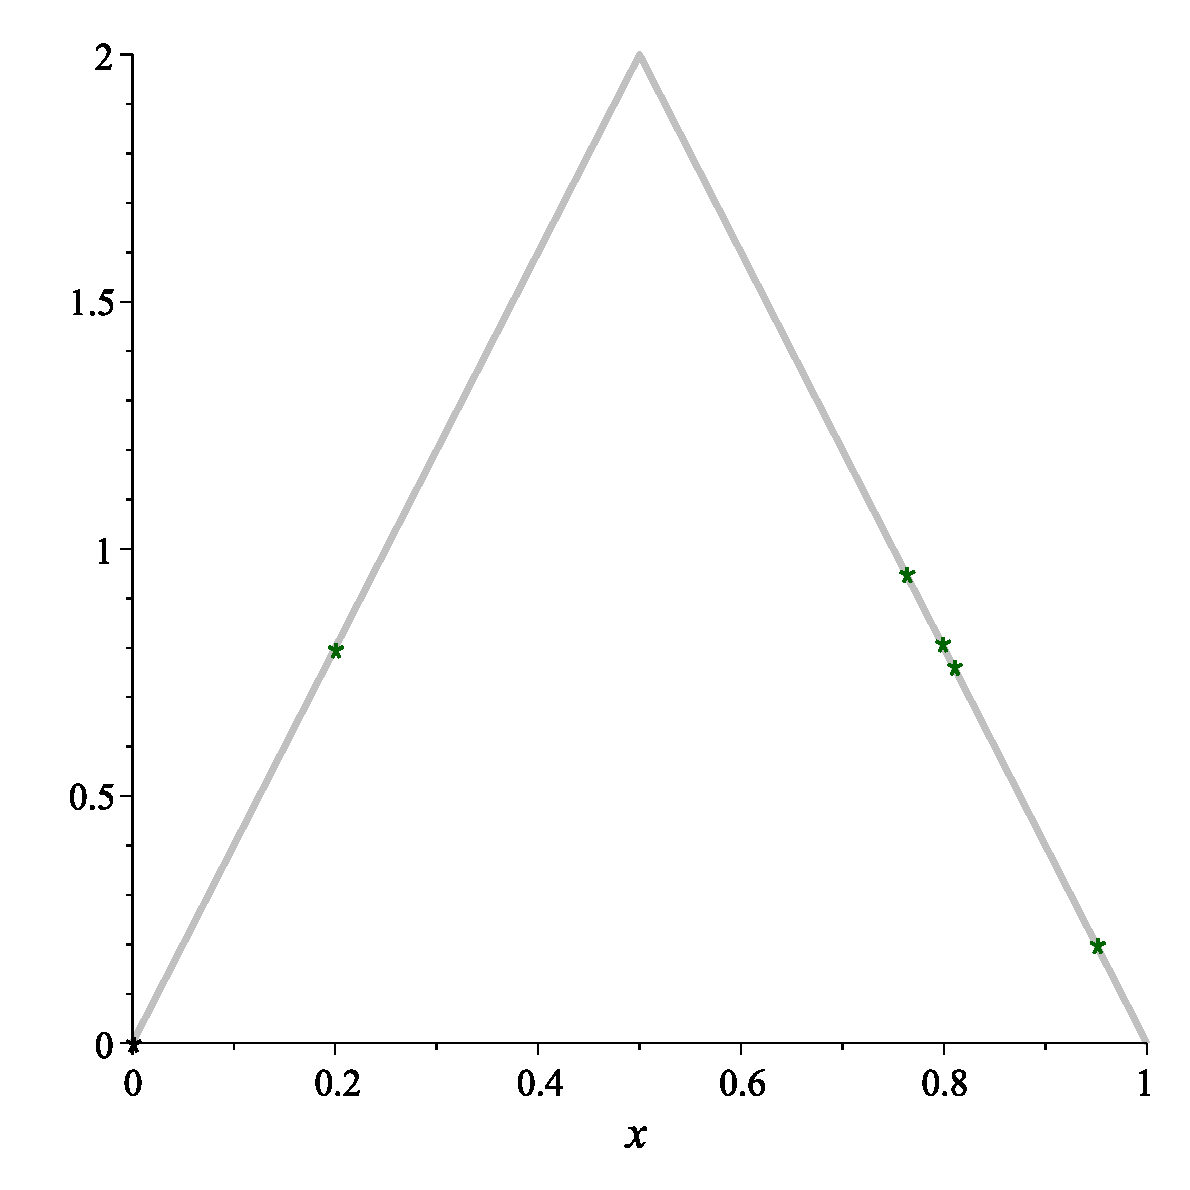
\includegraphics[scale=0.28]{Fig14b}
\caption{Cyclic points of 5-cycles and fixed points of the tent map in the case of positive (red and blue) and negative (green and black) multipliers} \label{f14}
\end{figure}

%_________________________________________________________________________________
\section{\centering{Distribution of cyclic points and visualization of the Cantor set}}

As noted above, the invariant set of equation~(\ref{eq}) at $H=3$ is the classical Cantor set. However, due to its strong instability, it is impossible to visualize 
the points of this set using equation~(\ref{eq}). The Cantor set is characterized by two types of points: the points that are end-points of the intervals adjacent to 
to the Cantor set are called points of the first type, while the other points of the set are called points of the second type. Points of the first type can be obtained 
as the union of all roots of the equations $f^{(k)}(x) = 1,$ $k=1,\,2,\ldots\,$. The set of points of the first type is countable. Among the points of the second type, we can select
a subset consisting of all cyclic points of map~(\ref{tent}). They are obtained as the union of all the roots of the equations $f^{(k)}(x) = x,$ $k=1,\,2,\ldots\,$. 
The set of cyclic points of map~(\ref{tent}) is also countable.

If an infinite number of points of the Cantor set lie between two points of the first type, then there also lie an infinite number of periodic points between them. 
Consequently, since each point of the Cantor set is a limit point for the set of points of the first type, then each point of the Cantor set will be limit for the set 
of cyclic points as well.

The following question arises: how are the periodic points of one orbit of a given period $T,$ of several such orbits located in the Cantor set? More precisely, how uniformly 
do the periodic points of the orbit of a given period $T$ fill the Cantor set? The paper does not consider the analytical solution of this problem, 
only some examples of visualization of the density functions for the distribution of periodic points are constructed, and they are graphically compared with 
the analogous function for a random sample of elements from the set of the first-type points of the Cantor set.

Let us take for example the period $T=1009,$ accuracy $10^{-525},$ initial value $x_0=0.555,$ values for the control parameter 
$\vartheta = \frac{H^T \pm \frac{0.6}{H}}{H^T + 1}.$ We will get $2T=2018$ cyclic points. Let us construct the density function for the distribution 
of the cyclic points set (Fig.~\ref{f15}-a). The graph shows that the found periodic points are not quite evenly distributed in the Cantor set. Let us now find \textit{two hundred} orbits with the period 
$T=1009,$ i.e., we get 20180 cyclic points. Surprisingly, the graph of the distribution density function for the new set of points (Figure~\ref{f15}-b) does not differ much 
from the plot in the previous case. Finally, let us plot the density function for the distribution of randomly selected 200000 points of the first type of the Cantor set.
For this purpose, represent the points from the set of the first type of the Cantor set in the form $s = \sum\limits_{j=1}^{N}{\alpha_j}{\frac{2}{3^j}},$ where 
the set $\left\{ \alpha_1,\ldots,\,\alpha_N\right\}$ consists of zeros and ones. Take $N=25.$ Then the maximum number of possible points is $2^{25}$. 
Let us randomly choose values for $\alpha_j$: either zero or one, and thus construct 200000 points. Next, we build a graph of the distribution density function 
of the resulting set (Fig.~\ref{f16}). Comparison of the graphs in Figures~\ref{f15}, \ref{f16} shows that the points of the first type, constructed by the above method, 
are distributed more evenly on the Cantor set. 
 
% Figure 15
\begin{figure}[h!]
\begin{minipage}[h]{0.45\linewidth}
\center{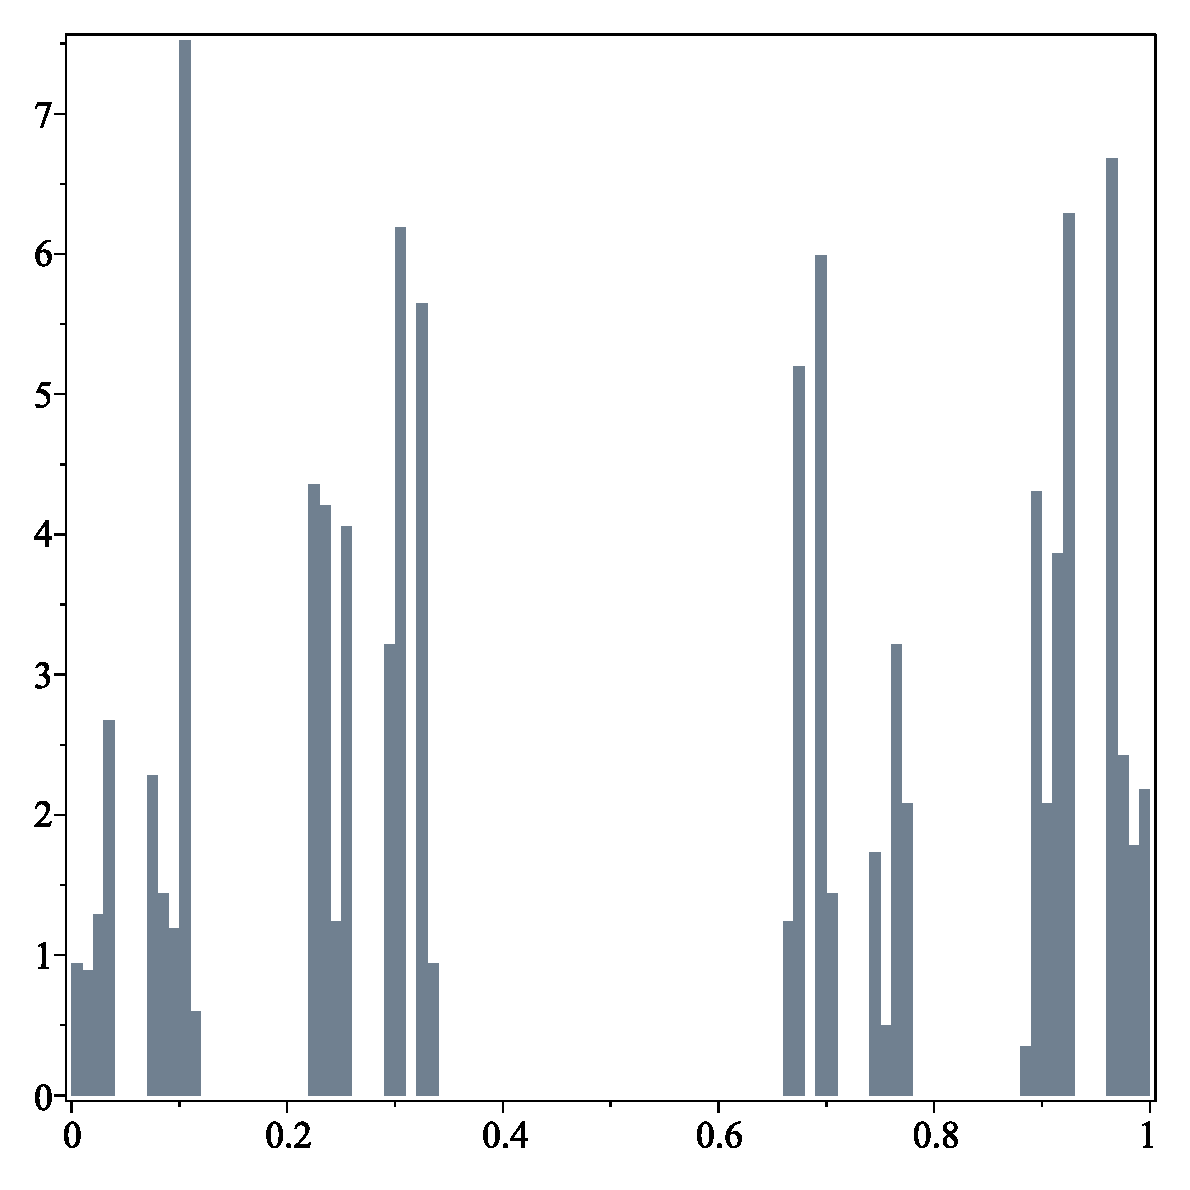
\includegraphics[scale=0.28]{Fig15a} \\ a)}
\end{minipage}
\hspace{1cm}
\begin{minipage}[h]{0.45\linewidth}
\center{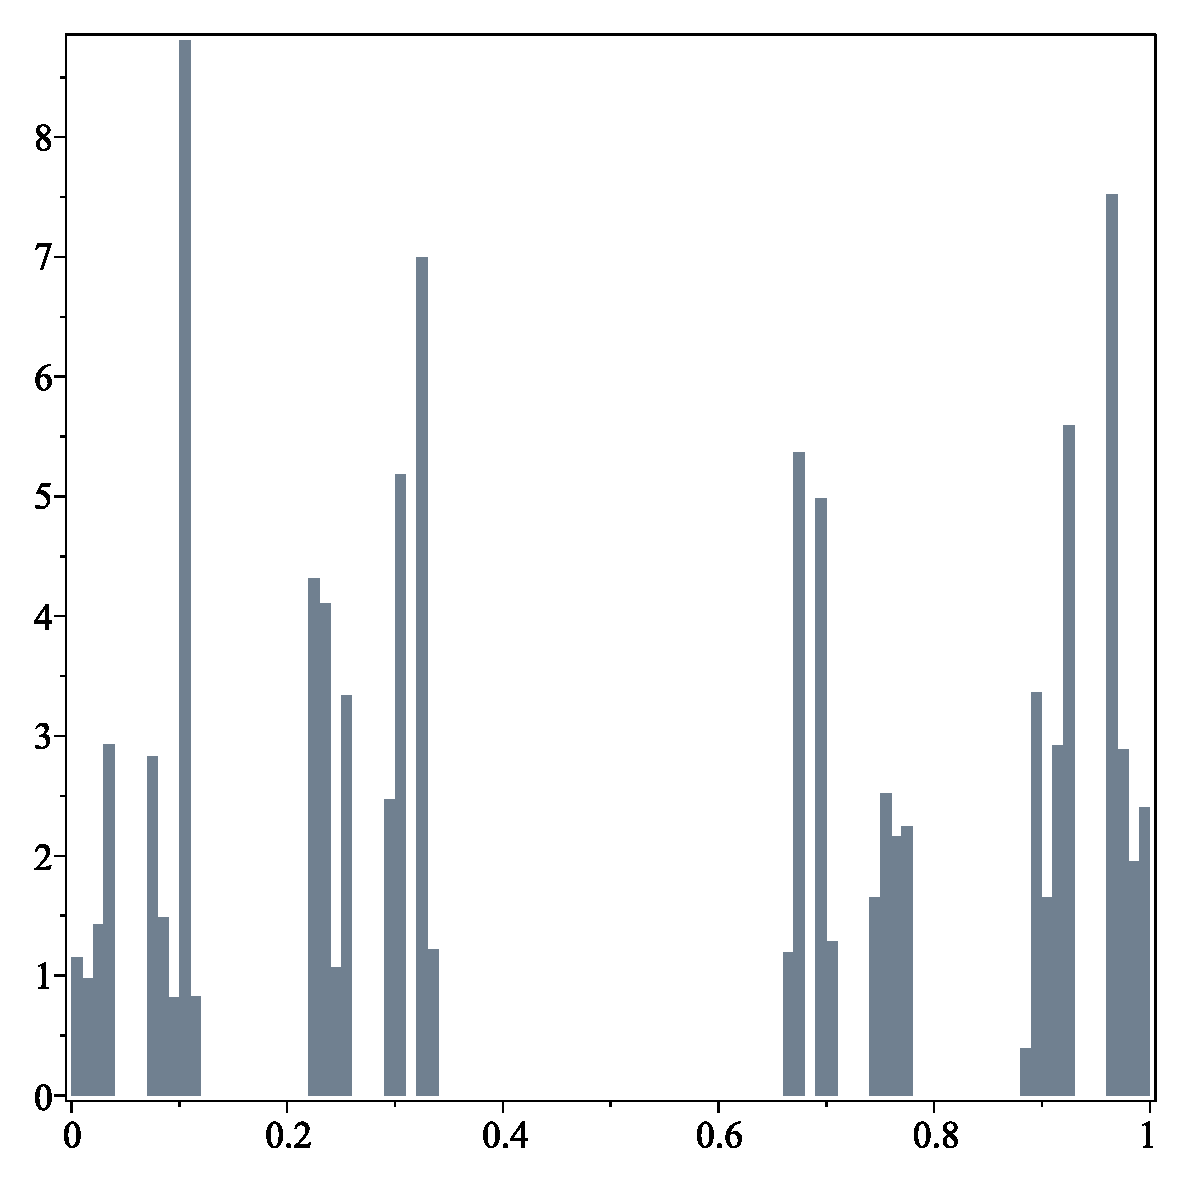
\includegraphics[scale=0.28]{Fig15b} \\ b)}
\end{minipage}
\caption{The graph of the distribution density function of the set of cyclic points of two and two hundred 1009-periodic orbits of map~(\ref{tent}) at $H=3$} \label{f15}
\end{figure}

% Figure 16
\begin{figure}[h!]
\centering
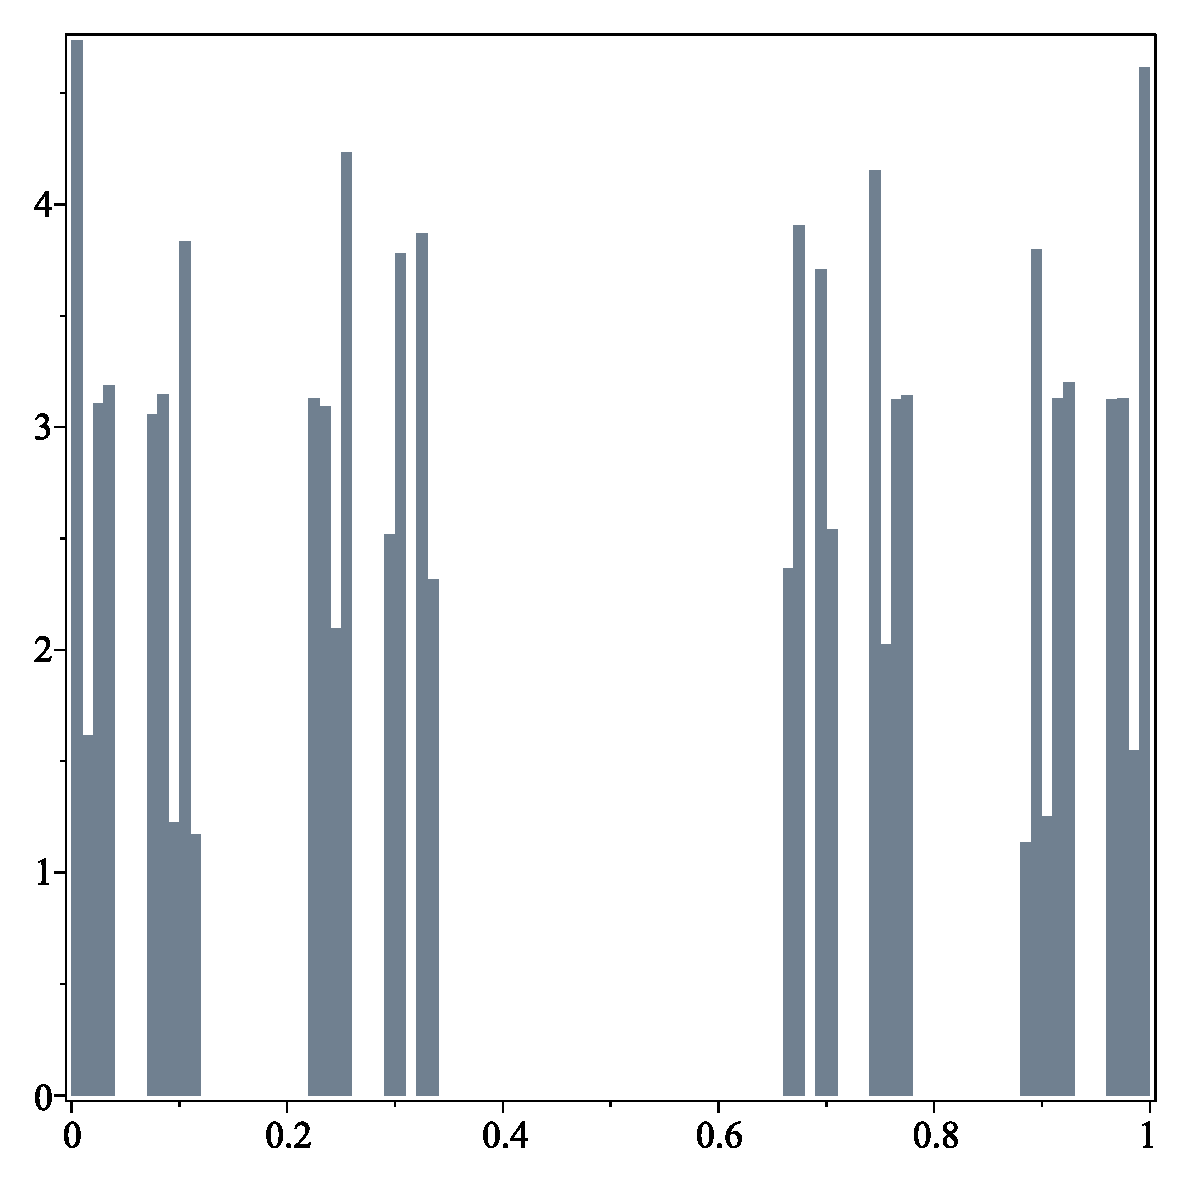
\includegraphics[scale=0.28]{Fig16}
\caption{Graph of the distribution density function of the set of 200000 random points of the first type of the Cantor set} \label{f16}
\end{figure}

%_________________________________________________________________________________
\section{\centering{Conclusions}}

In \cite{DSI}, there was solved the problem of constructing the framework of the nonlinear dynamic systems attractor through a set of the periodic orbits, which were 
found using generalized predictive control. If the invariant set is a repeller, then the analogous problem turns out to be much more complicated: simple local stability 
of the orbit is not sufficient, due to the fact that the basin of attraction can have a small measure, and for most of the initial points the trajectory will go to infinity. 
However, the method of generalized predictive control, used to stabilize the orbit, has an important characteristic: in addition to the local asymptotic stability 
of the orbits of controlled motion, the rest of the orbits remain bounded for a sufficiently large set of initial values. For the generalized tent map, it is possible to ensure 
that all the solutions are bounded. The global behavior of solutions for the generalized logistic map, the generalized Lozi \cite{Lozi1} and H\'enon maps, etc. is somewhat more complicated. 
For such systems, apparently, it is necessary to choose the control parameter as a function of the current state of the system. Investigation of the global behavior of 
the controlled systems solutions for the mentioned maps is the task for future research.


\bibliographystyle{unsrt}
\bibliography{tentbib}

\end{document}